\documentclass[a4paper]{article}

\usepackage{fullpage} % Package to use full page
\usepackage{parskip} % Package to tweak paragraph skipping
\usepackage{tikz} % Package for drawing
\usepackage{amsmath}
\usepackage{hyperref}

\title{Windows Server: SQL Server}
\author{Jens Du Four}
\date{2018 - 2019}

\begin{document}

\maketitle

\section{Introductie}
U bent IT-Consultant en krijgt de vraag om een voorstel te maken en te demonstreren van een Windowsomgeving. Deze omgeving moet bestaan uit het volgende . De cliënt wenst een redundante oplossing voor zijn servers. Dit vooral op de domeincontrollers. De cliënt wenst ook dat er een mailomgeving geïnstalleerd wordt en een omgeving die toelaat om op een efficiënte manier Windows toestellen te installeren en te deployen.

\begin{center}
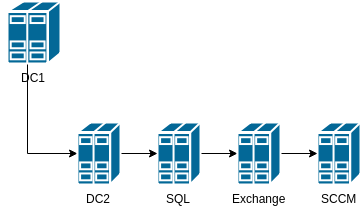
\includegraphics[width=8cm]{Netwerkdiagram.png}
\end{center}

\section{Server Requirements}

\begin{enumerate}
\item DC1
    \begin{enumerate}
    \item RAM: 2048 MB
    \item HDD: 50 GB
    \item Netwerkadapters: NAT en Internal Network (jenduf.gent)
            \begin{enumerate}
            \item NAT
            \end{enumerate}
            \begin{enumerate}
            \item IP: 192.168.1.1
            \item SN: 255.255.255.0
            \end{enumerate}
    \item OS Version: Windows Server 2016 
    \end{enumerate}
    
\clearpage

\item DC2
    \begin{enumerate}
    \item RAM: 2048 MB
    \item HDD: 50 GB
    \item Netwerkadapters: Internal Network (jenduf.gent)
            \begin{enumerate}
            \item IP: 192.168.1.2
            \item SN: 255.255.255.0
            \item DG: 192.168.1.1
            \end{enumerate}
    \item OS Version: Windows Server 2016 
    \end{enumerate}
    
\item SQL Server
    \begin{enumerate}
    \item RAM: 2048 MB
    \item HDD: 50 GB
    \item Netwerkadapters: Internal Network (jenduf.gent)
            \begin{enumerate}
            \item IP: 192.168.1.3
            \item SN: 255.255.255.0
            \item DG: 192.168.1.1
            \end{enumerate}
    \item OS Version: Windows Server 2016
    \item SQL Version: SQL Server 2013-2016
    \end{enumerate}
\item Exchange Server
    \begin{enumerate}
    \item RAM: 8096 MB
    \item HDD: 100 GB
    \item Netwerkadapters: Internal Network (jenduf.gent)
            \begin{enumerate}
            \item IP: 192.168.1.4
            \item SN: 255.255.255.0
            \item DG: 192.168.1.1
            \end{enumerate}
    \item OS Version: Windows Server 2016
    \item Exchange Version: Exchange Server 2013-2016
    \end{enumerate}
\item SCCM Server
    \begin{enumerate}
    \item RAM: 8089 MB
    \item HDD: 100 GB
    \item Netwerkadapters: Internal Network (jenduf.gent)
            \begin{enumerate}
            \item IP: 192.168.1.5
            \item SN: 255.255.255.0
            \item DG: 192.168.1.1
            \end{enumerate}
    \item OS Version: Windows Server 2016
    \item OS Version: Windows Deployment Server 2012
    \end{enumerate}
\end{enumerate}

\section{Windows Server Installatie}
\begin{center}
	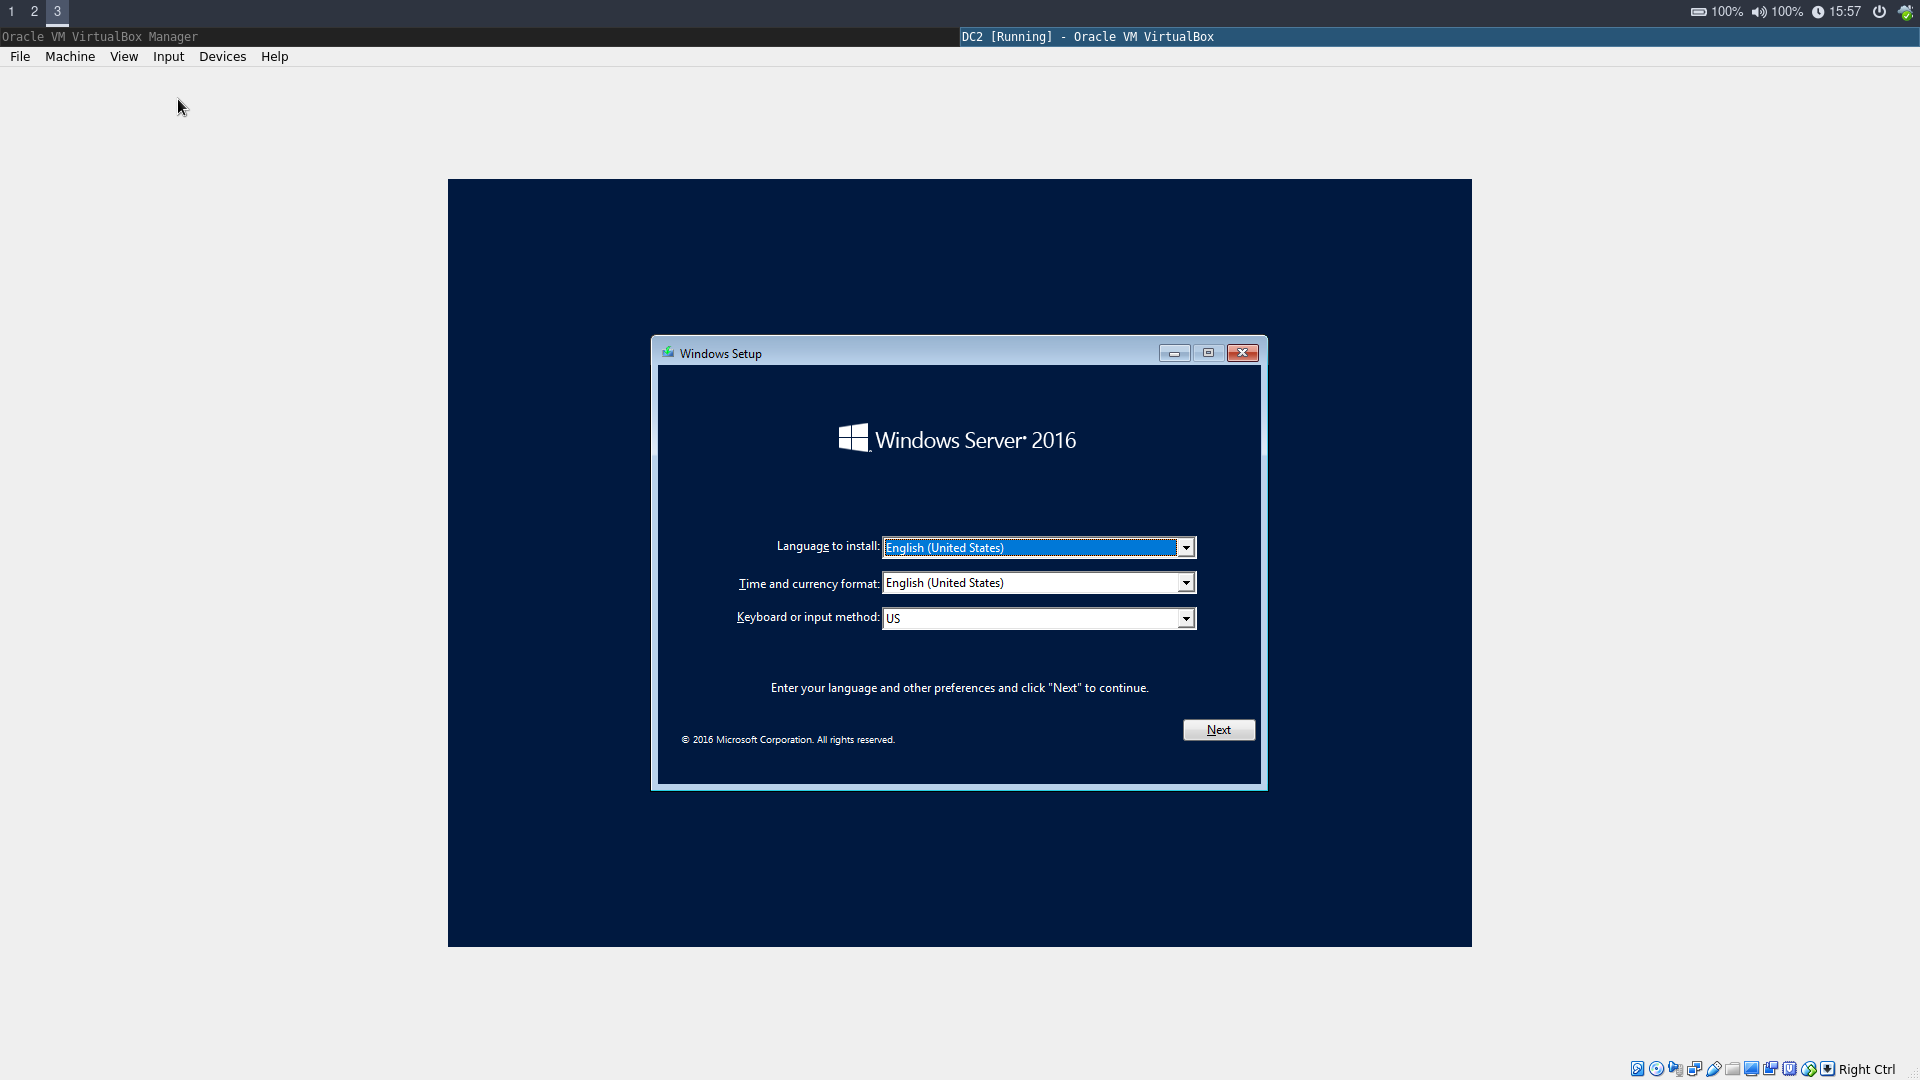
\includegraphics[width=15cm]{Pictures/Windows_Install/1542293852.png}
	Selecteer de gewenste taalinstellingen.
\end{center}
\begin{center}
	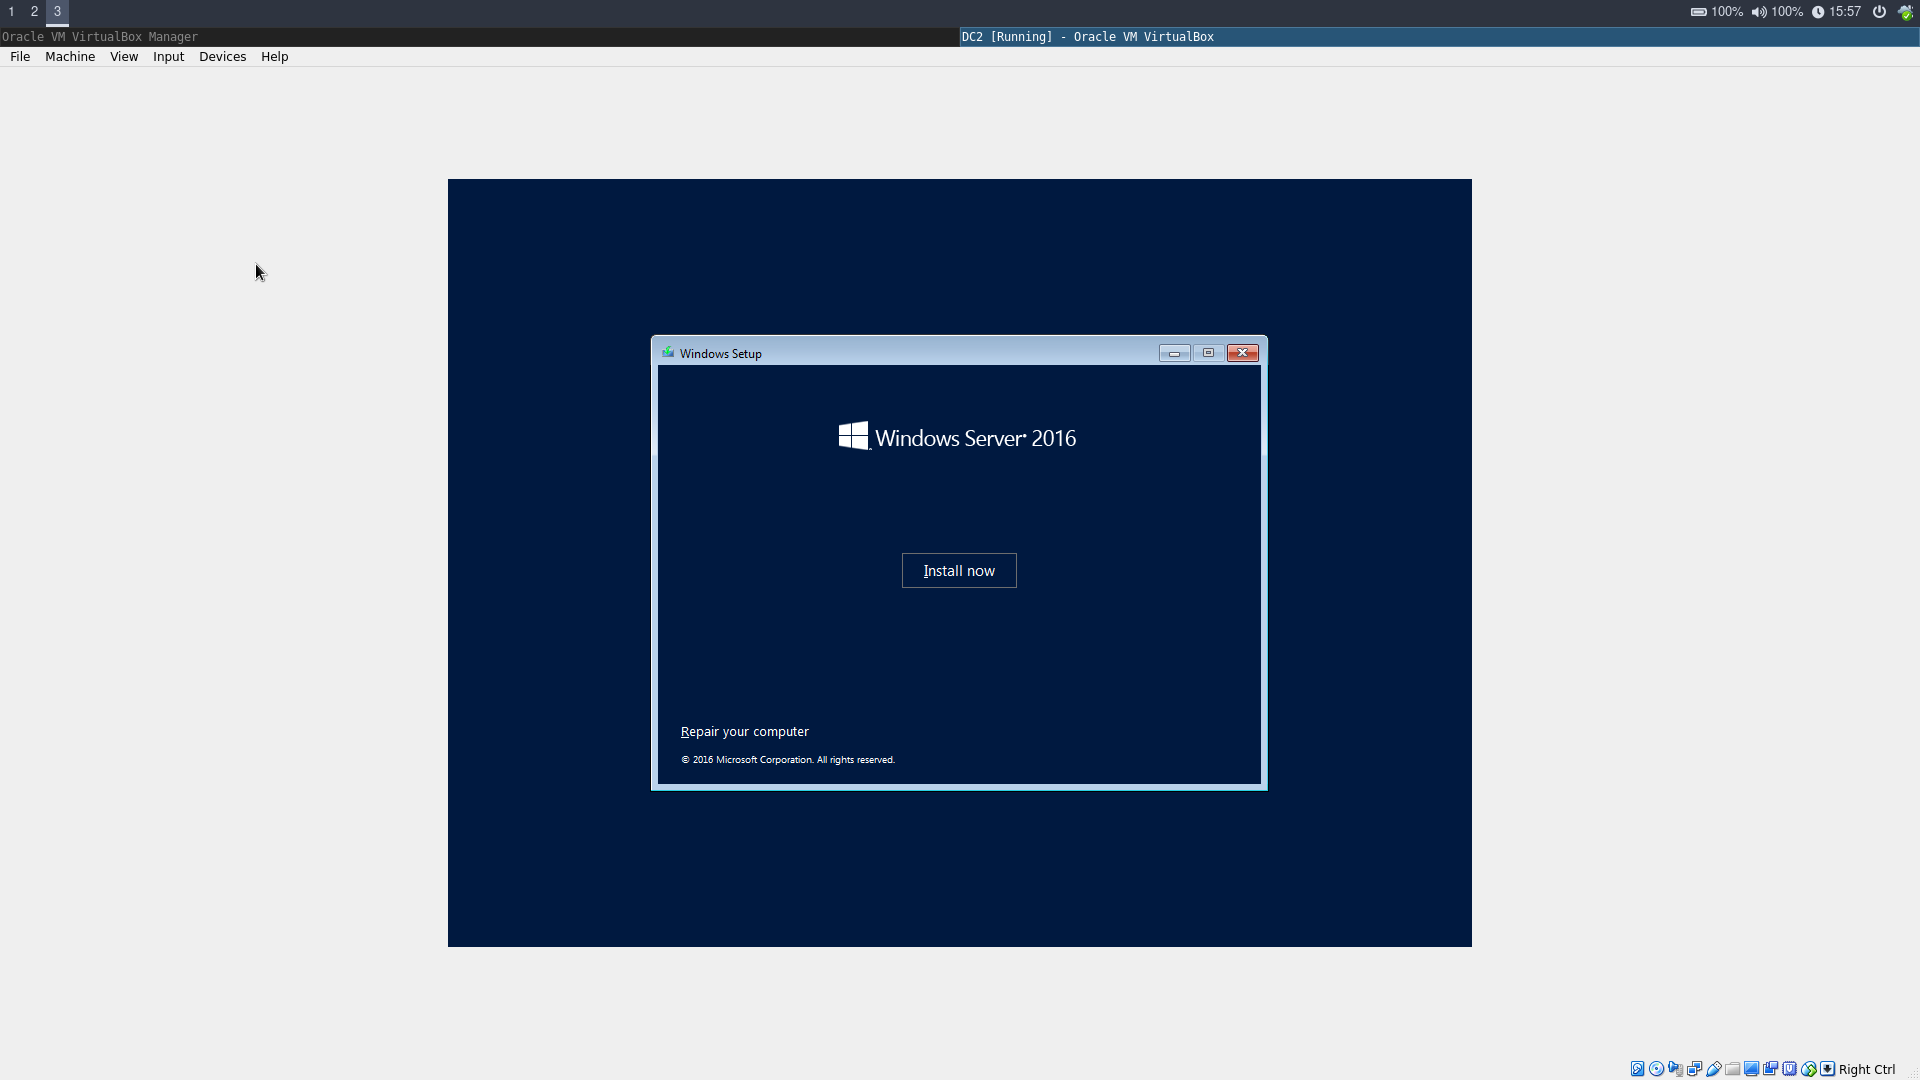
\includegraphics[width=15cm]{Pictures/Windows_Install/1542293872.png}
	
	Start de installatie.
\end{center}
\begin{center}
	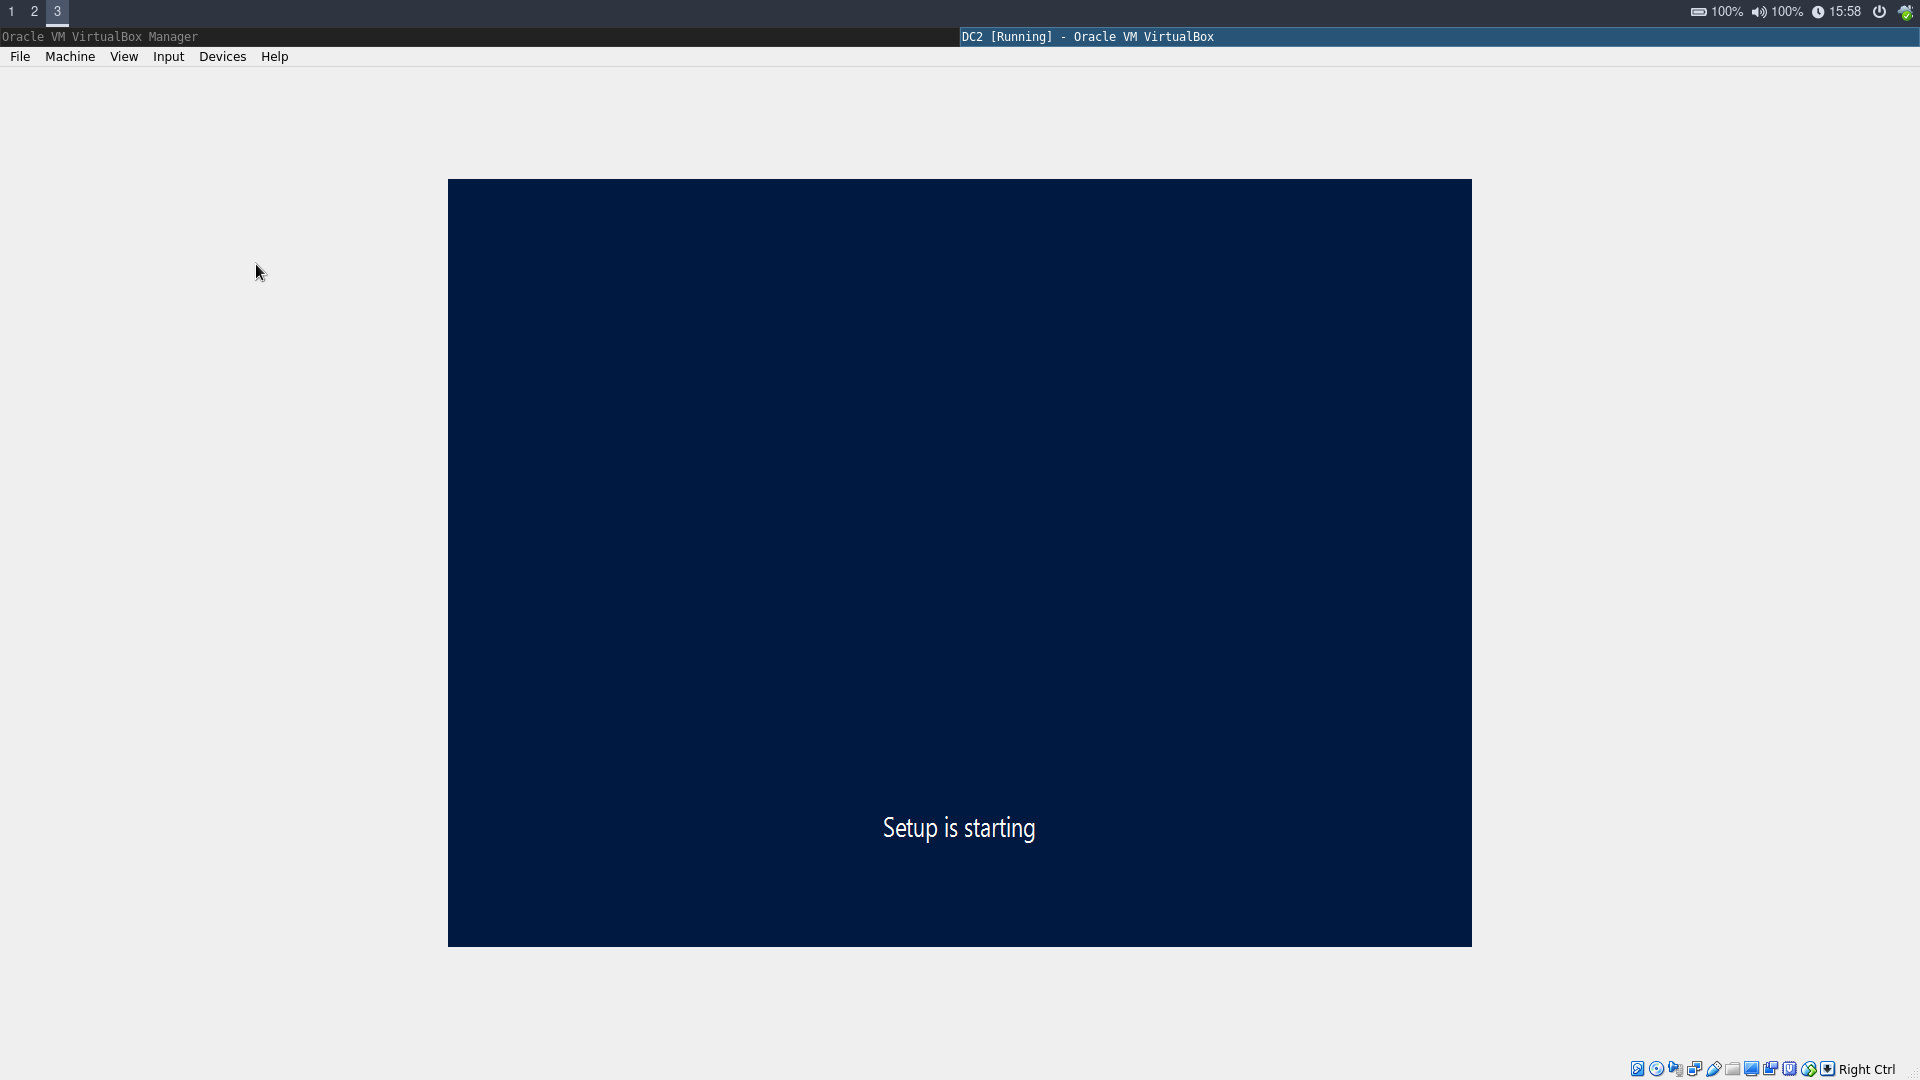
\includegraphics[width=15cm]{Pictures/Windows_Install/1542293887.png}
\end{center}
\begin{center}
	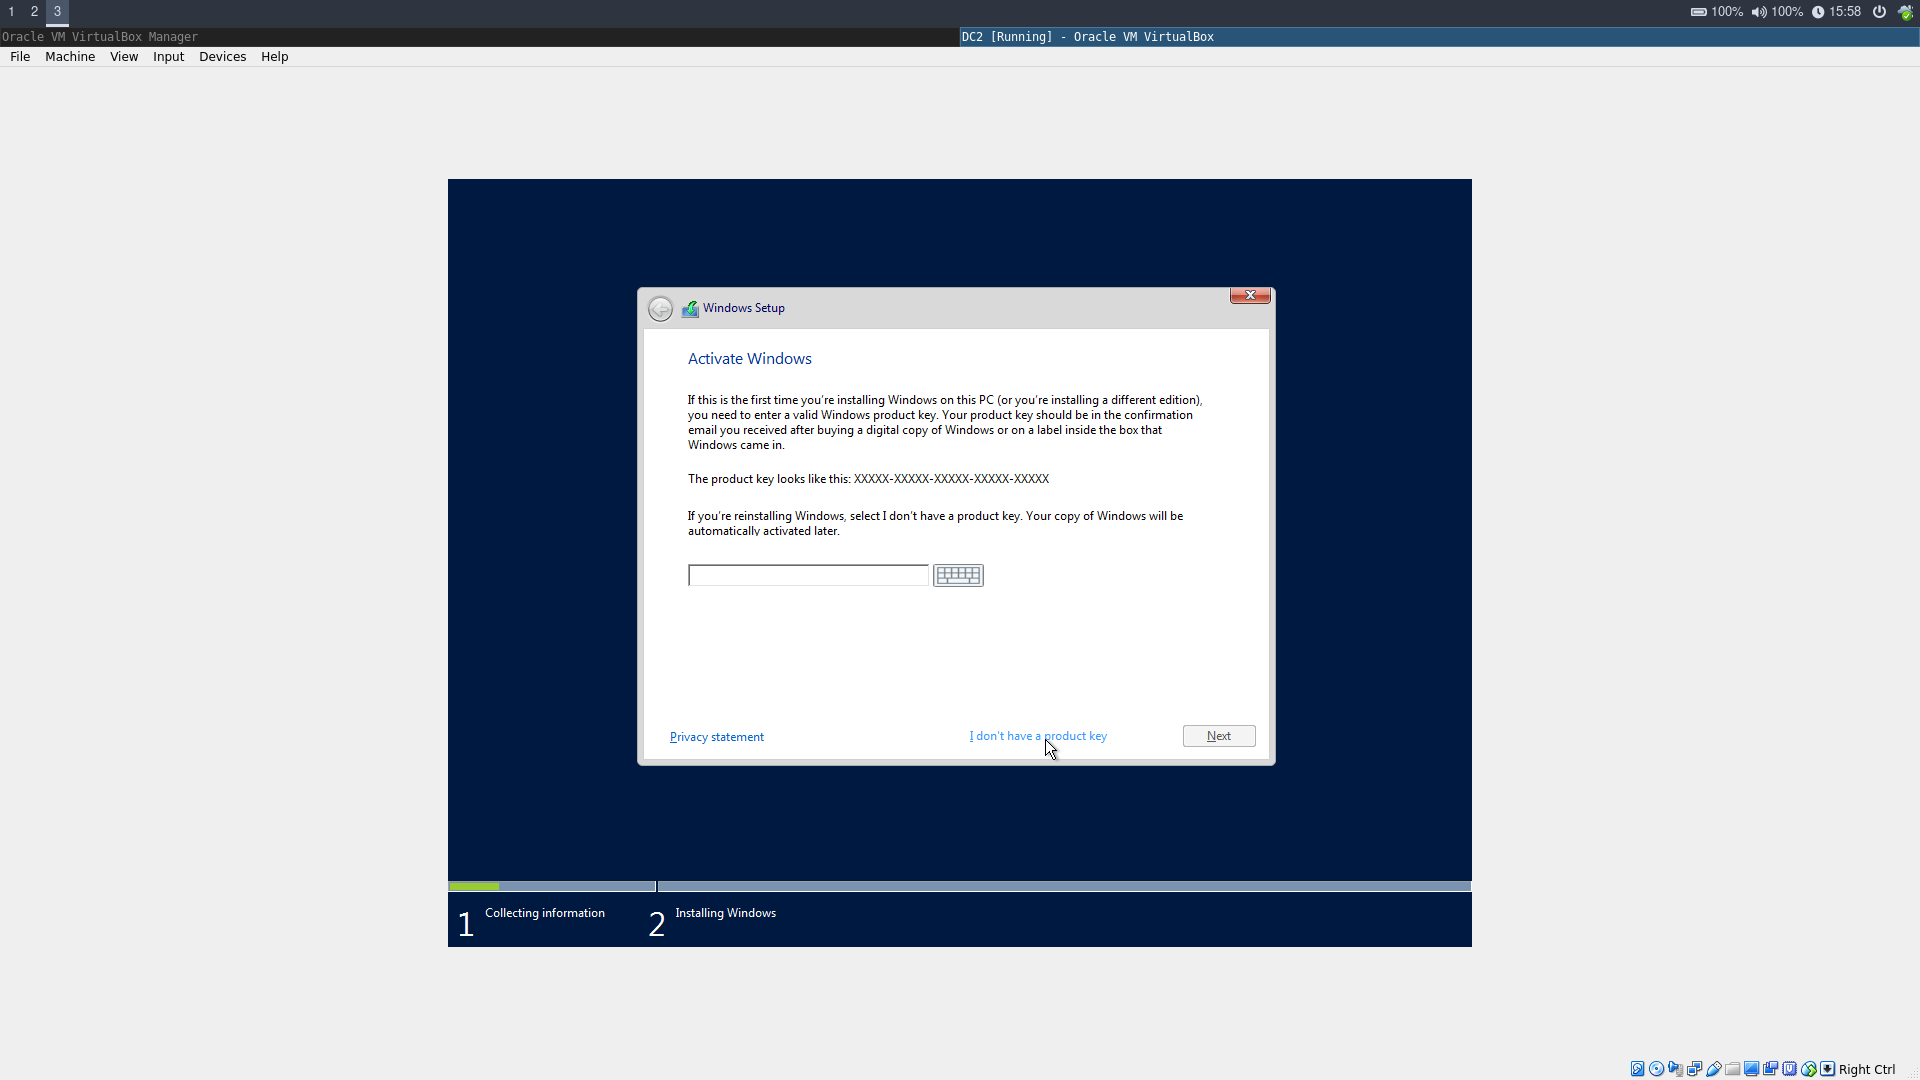
\includegraphics[width=15cm]{Pictures/Windows_Install/1542293899.png}
	
	Selecteer "I don't have a product key".
\end{center}
\begin{center}
	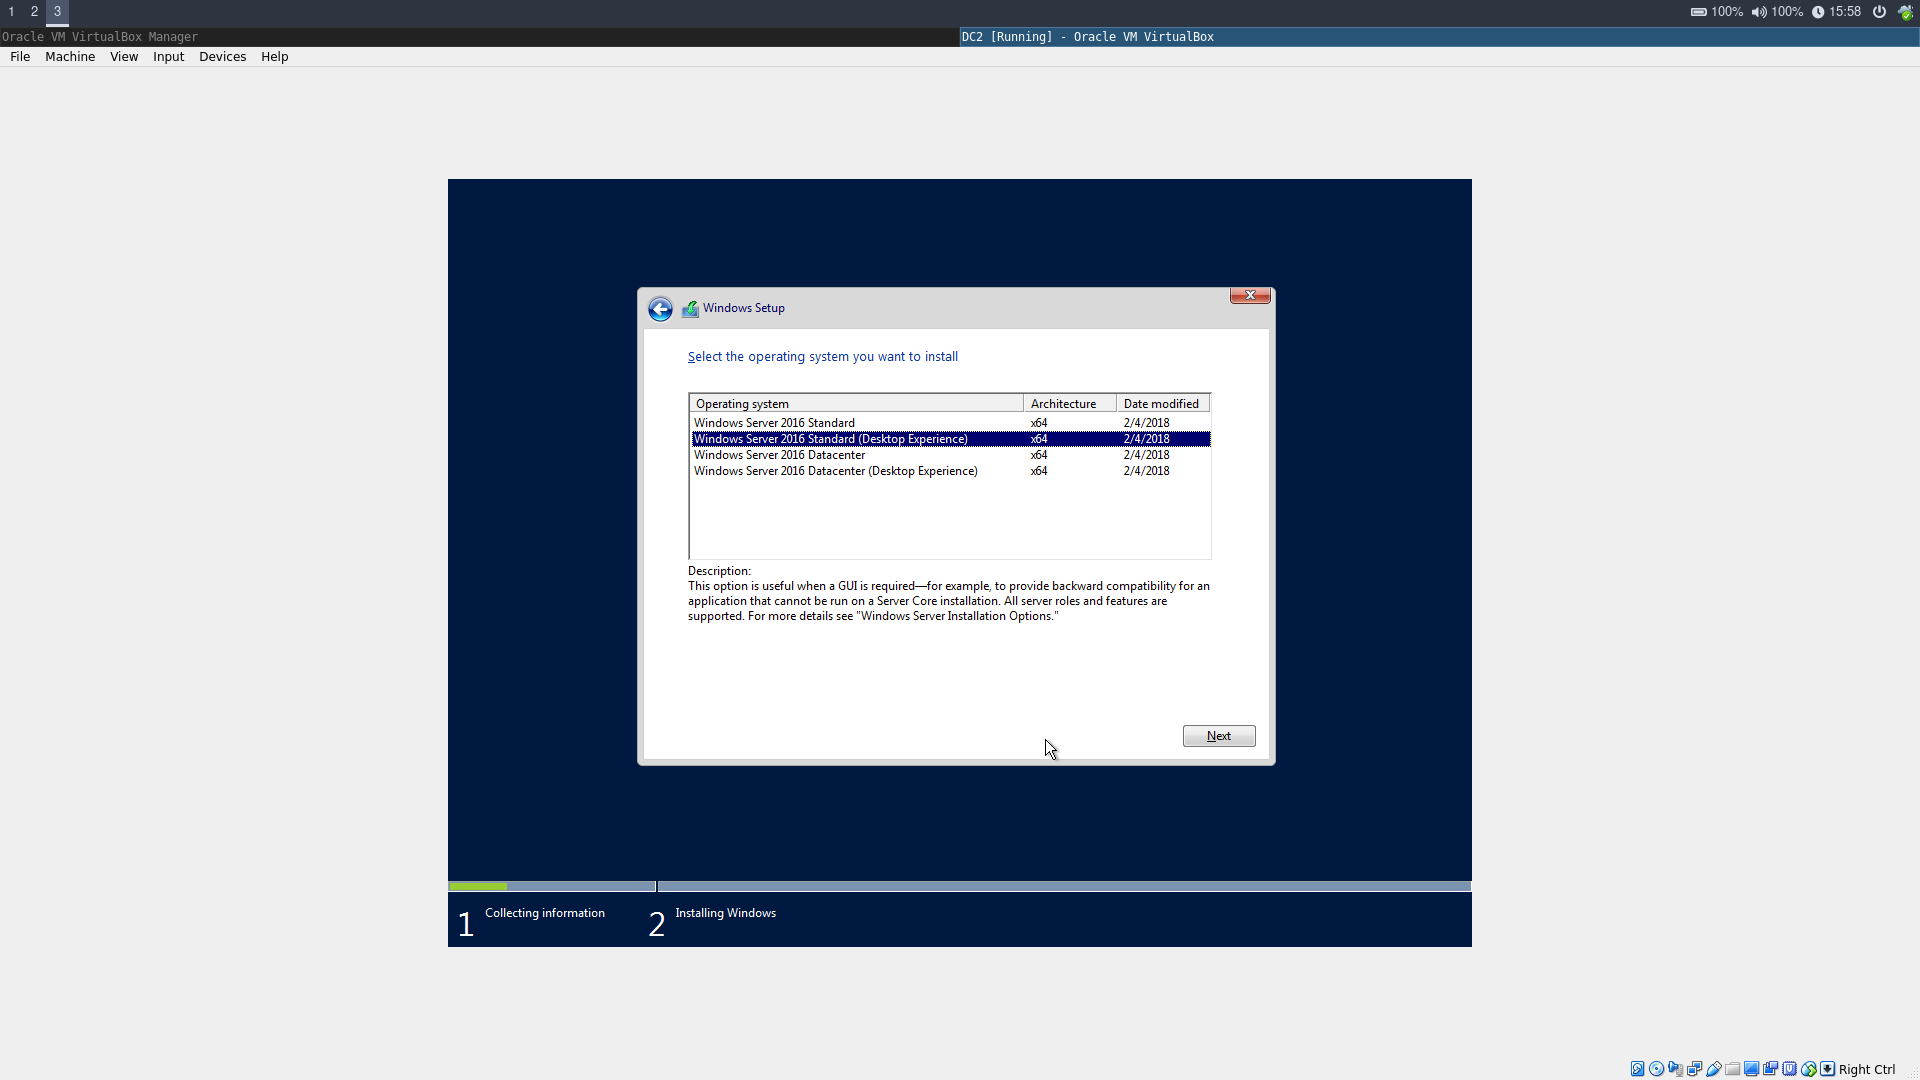
\includegraphics[width=15cm]{Pictures/Windows_Install/1542293908.png}
	
	Selecteer "Windows Server 2016 Standard (Desktop Experience)".
\end{center}
\begin{center}
	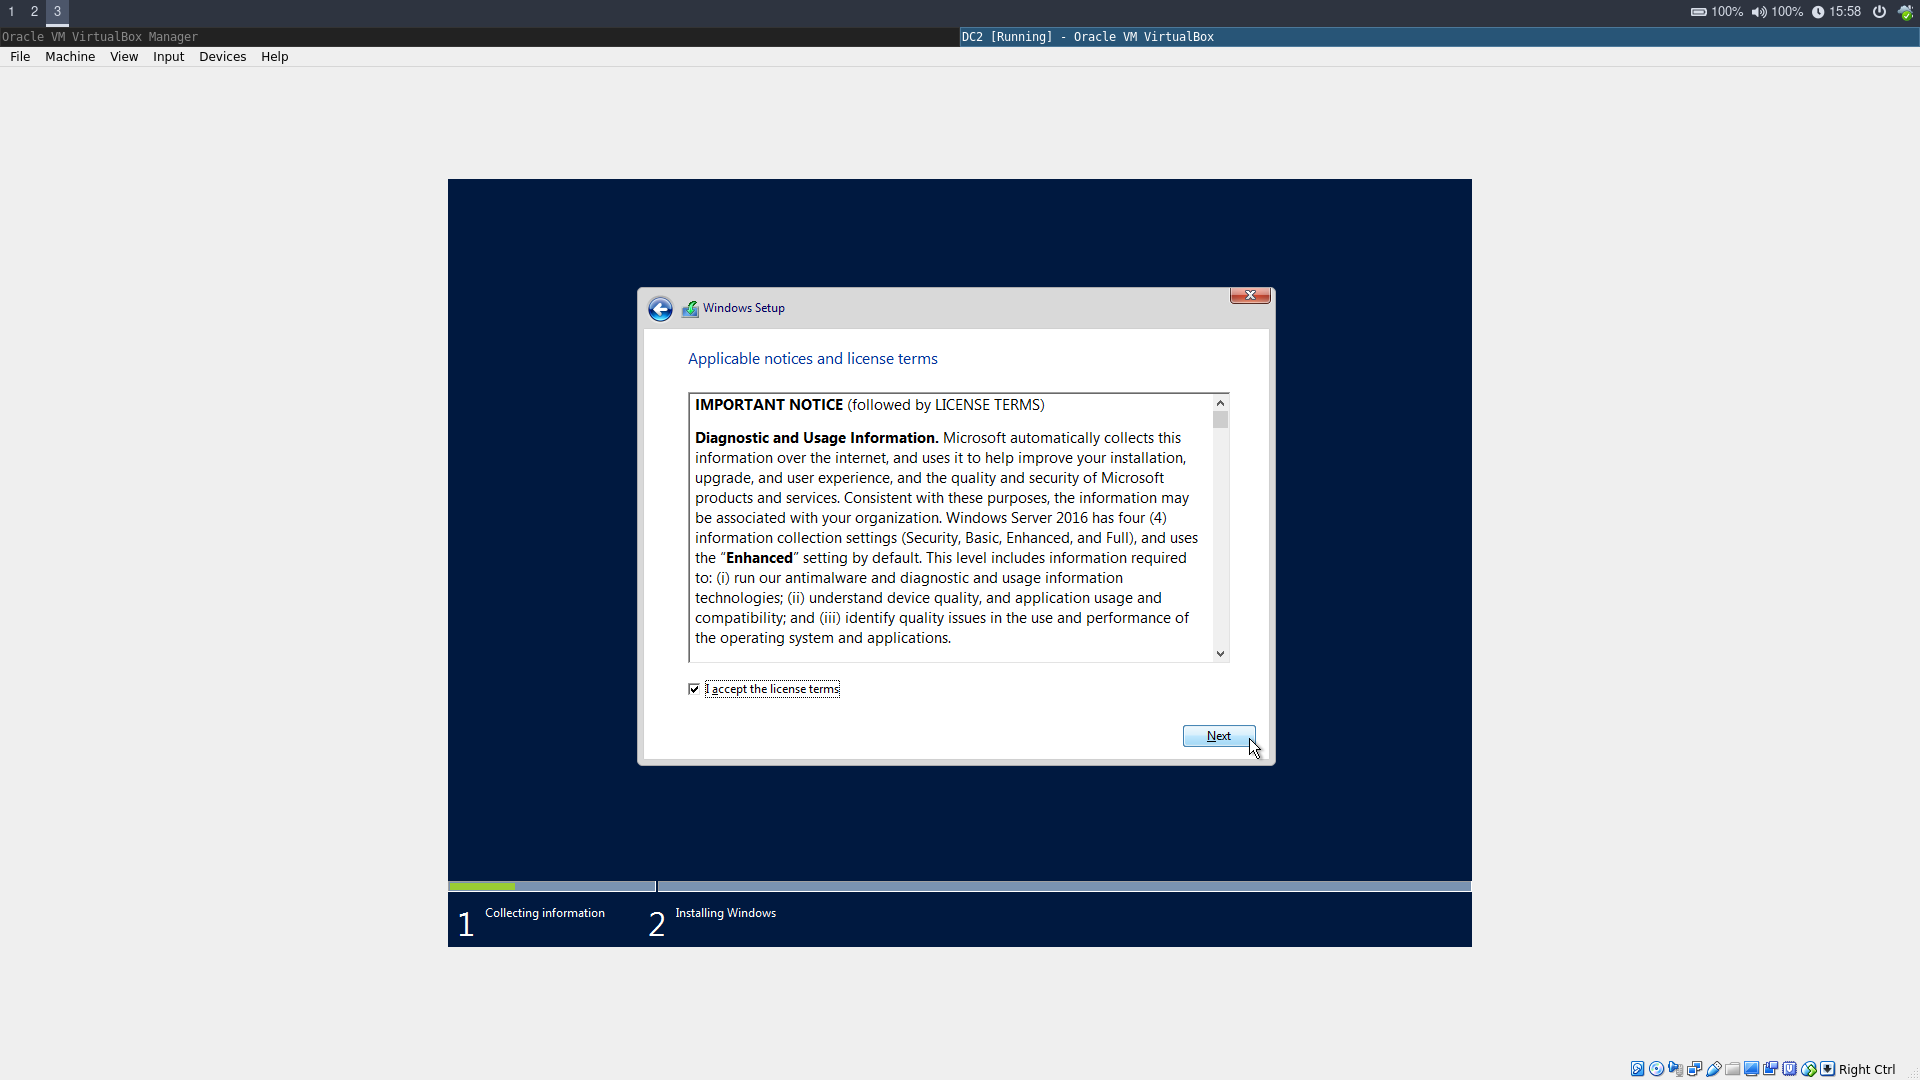
\includegraphics[width=15cm]{Pictures/Windows_Install/1542293921.png}
	
	Ga akkoord met de gebruiksvoorwaarden.
\end{center}
\begin{center}
	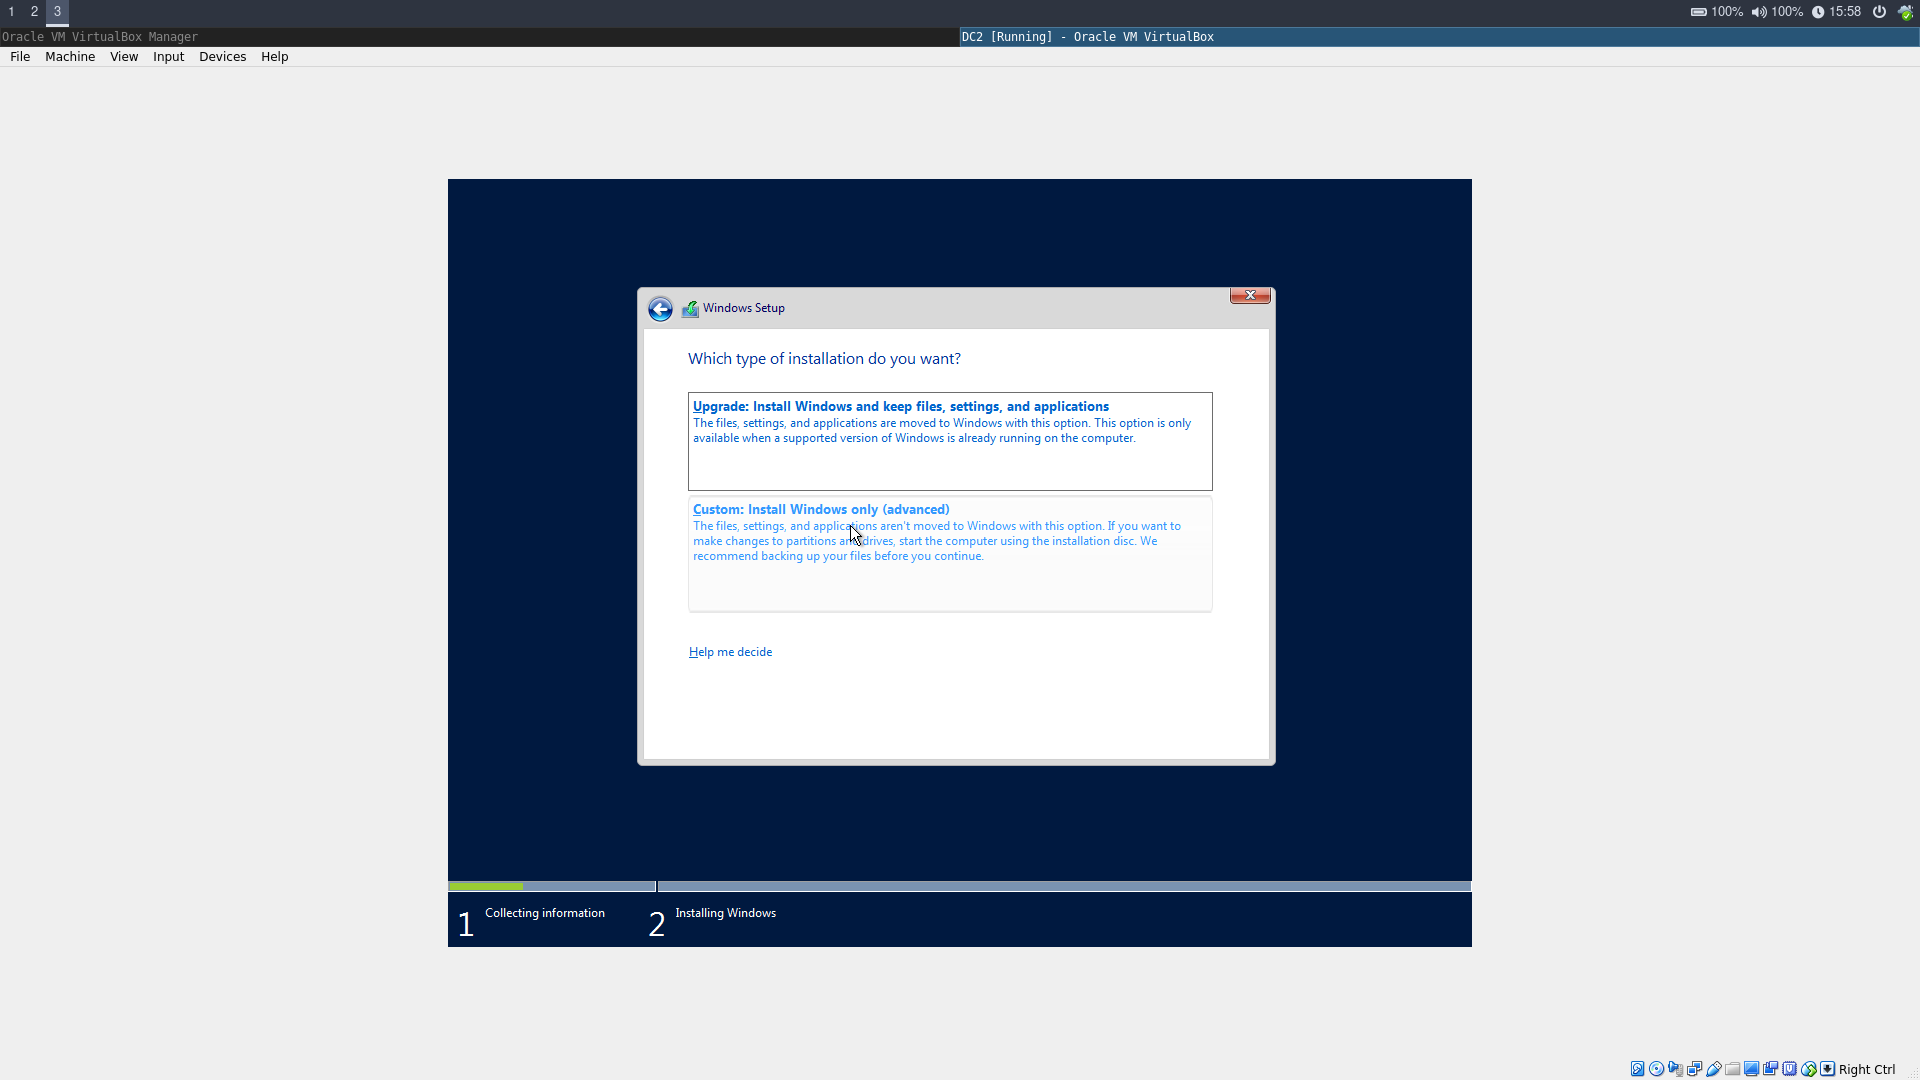
\includegraphics[width=15cm]{Pictures/Windows_Install/1542293929.png}
	
	Selecteer "Costum: Install Windows only (Advanced)".
\end{center}
\begin{center}
	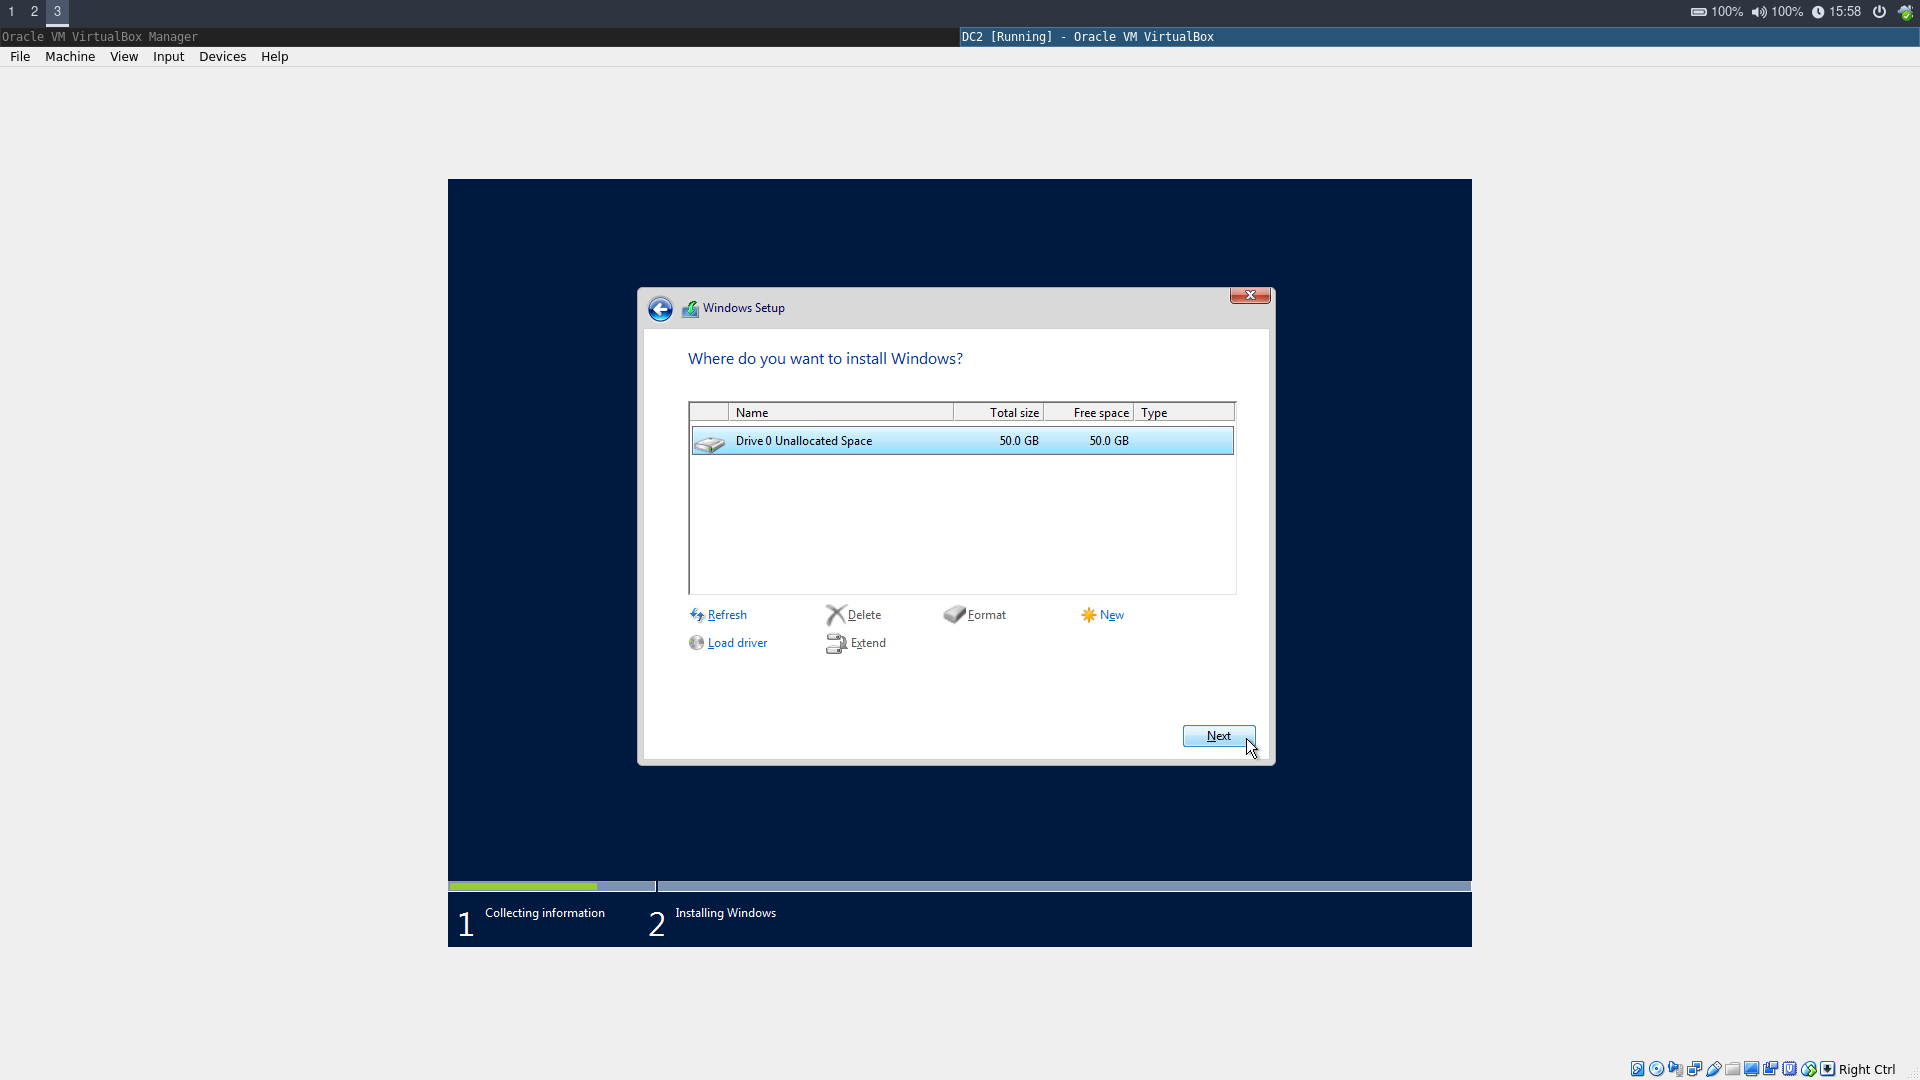
\includegraphics[width=15cm]{Pictures/Windows_Install/1542293934.png}
	
	Ga verder.
\end{center}
\begin{center}
	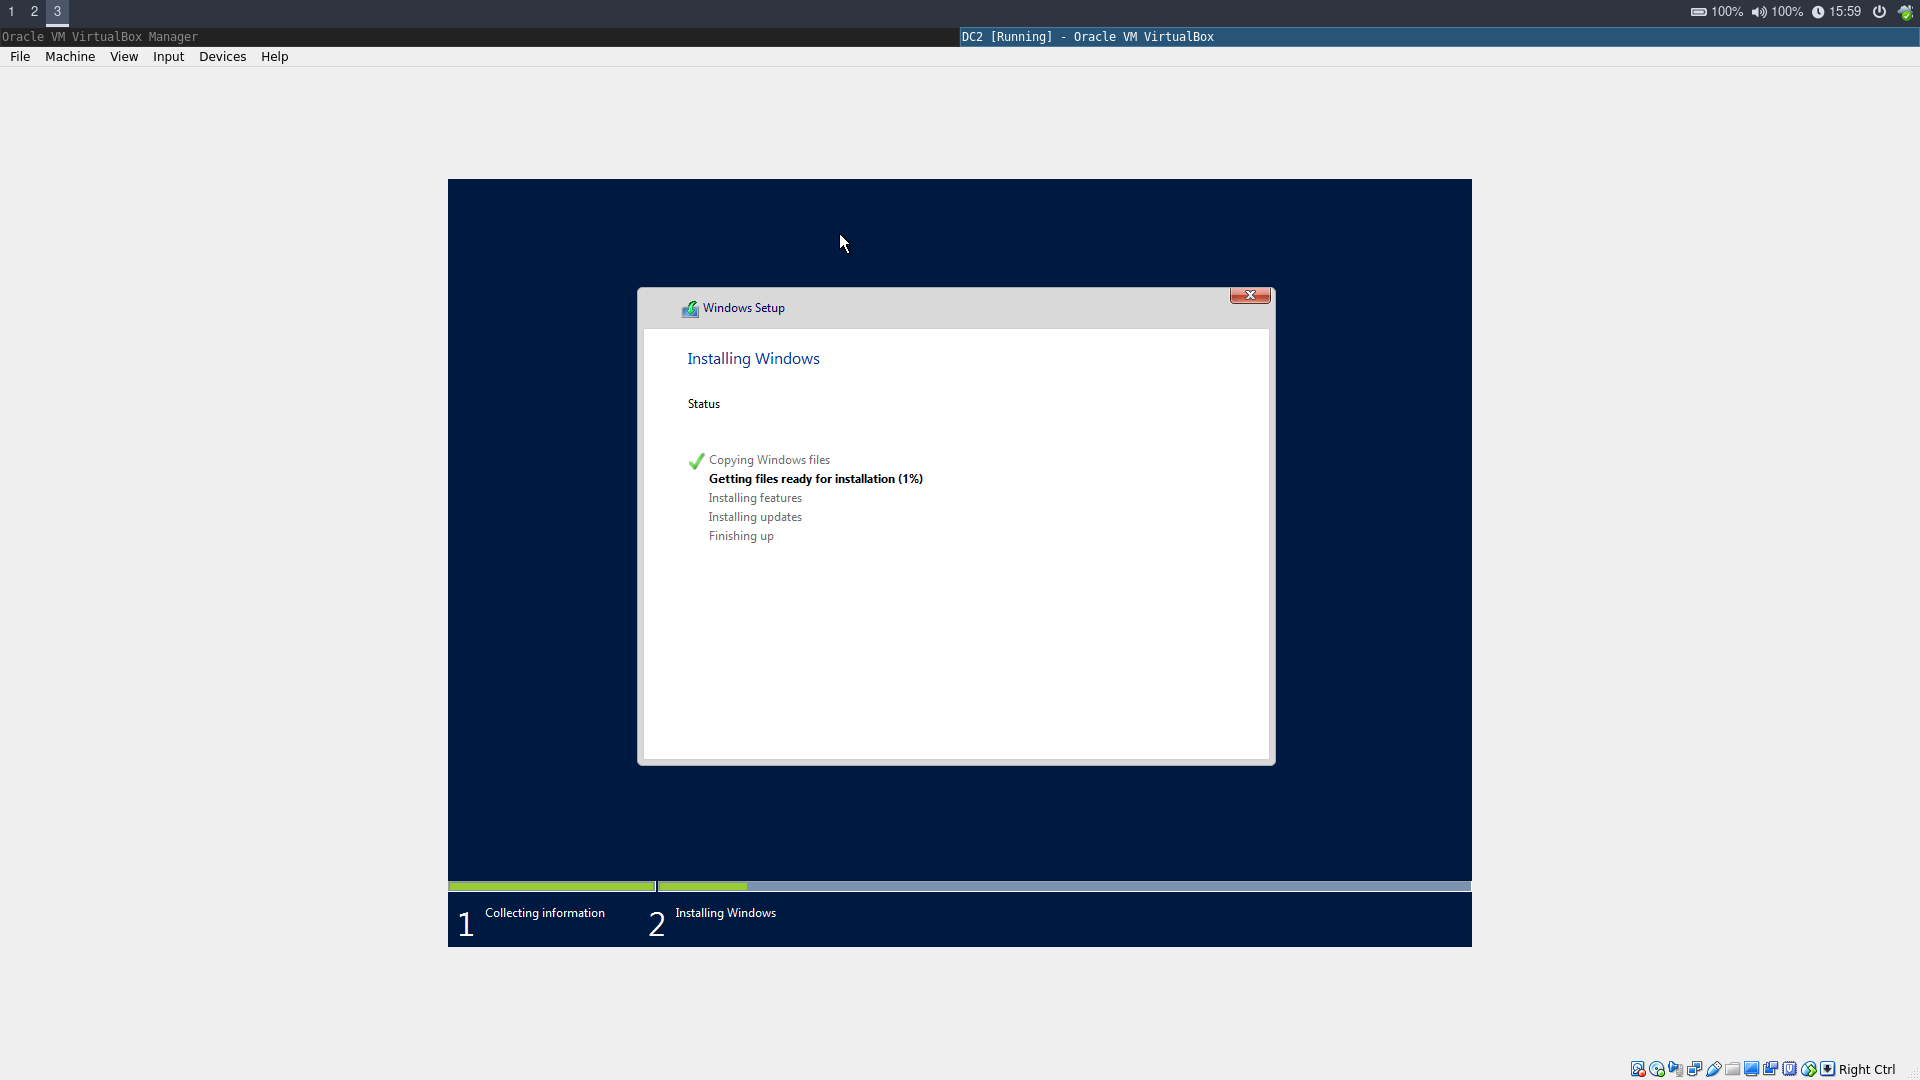
\includegraphics[width=15cm]{Pictures/Windows_Install/1542293945.png}
\end{center}
\subsection{Server Hernoemen}
\begin{center}
	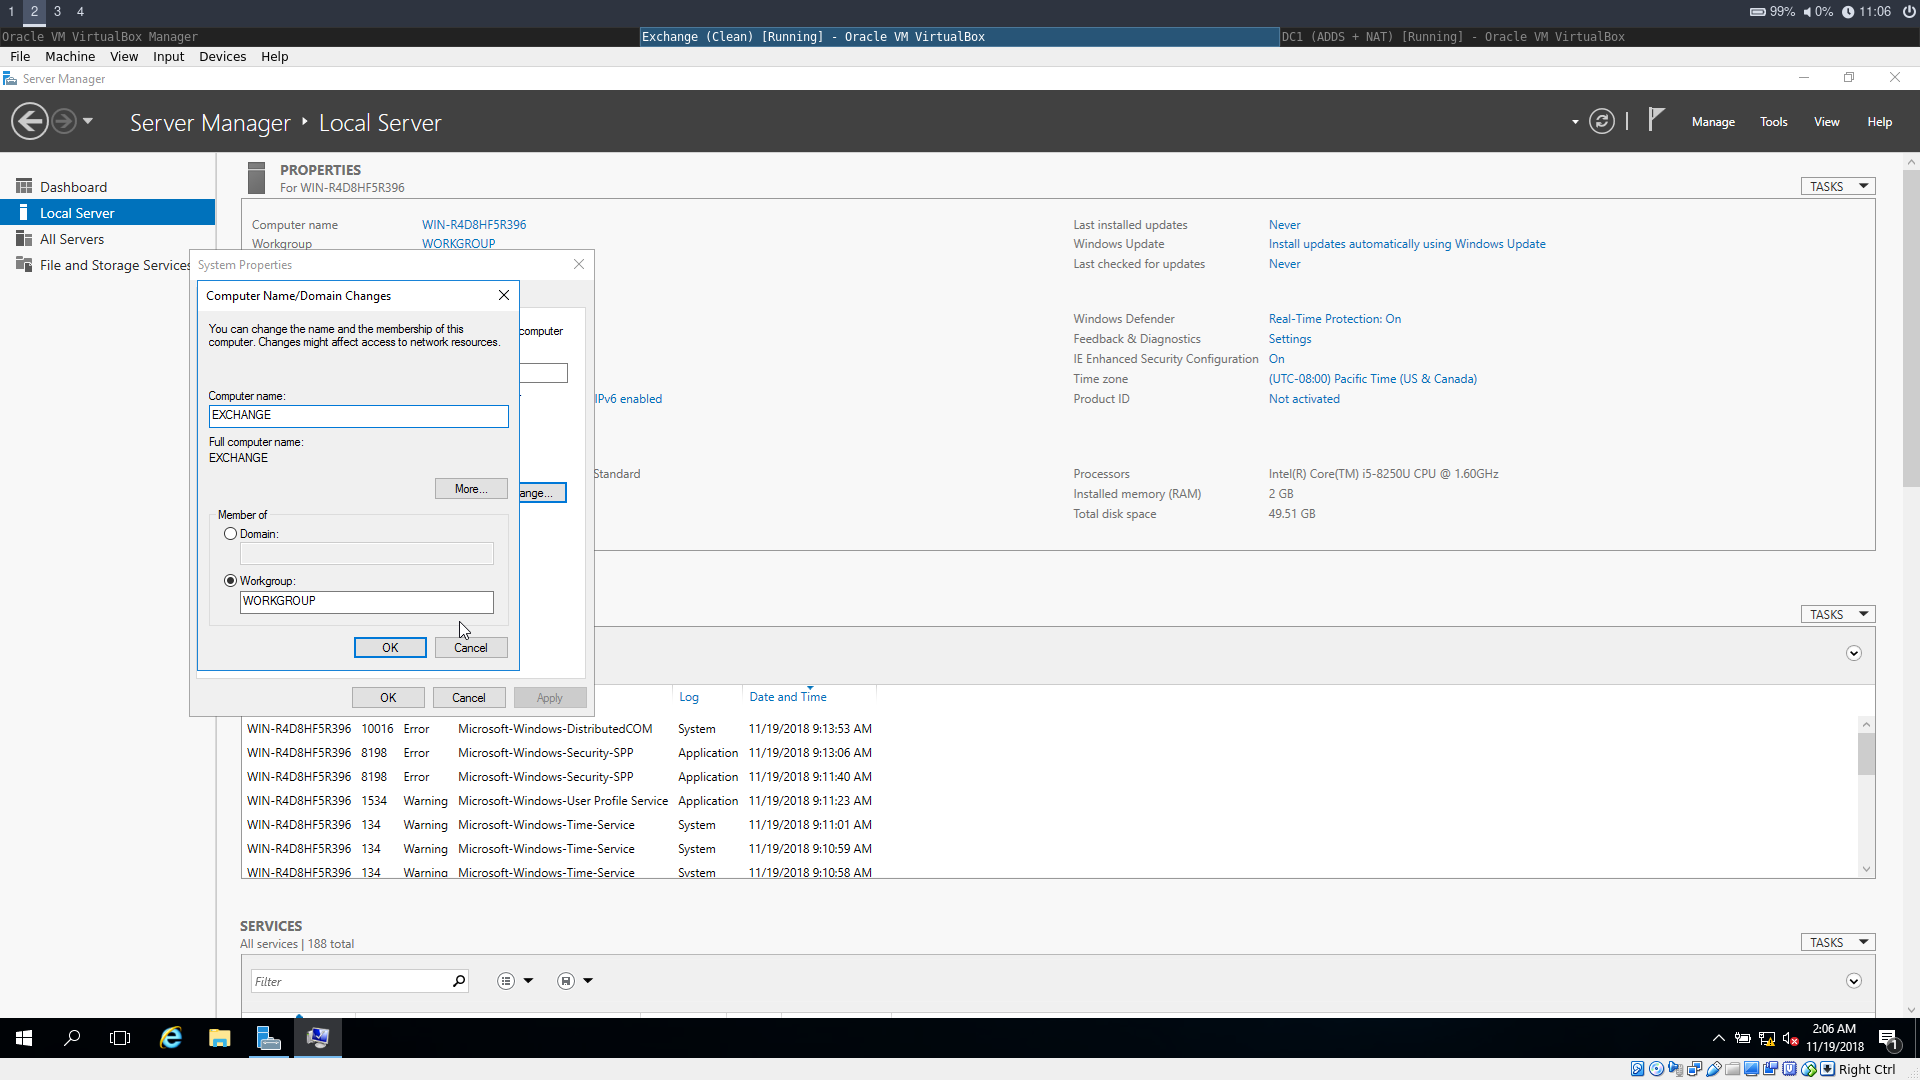
\includegraphics[width=15cm]{Pictures/Exchange/1542621993.png}
\end{center}
\subsection{IP Instellingen}
\begin{center}
	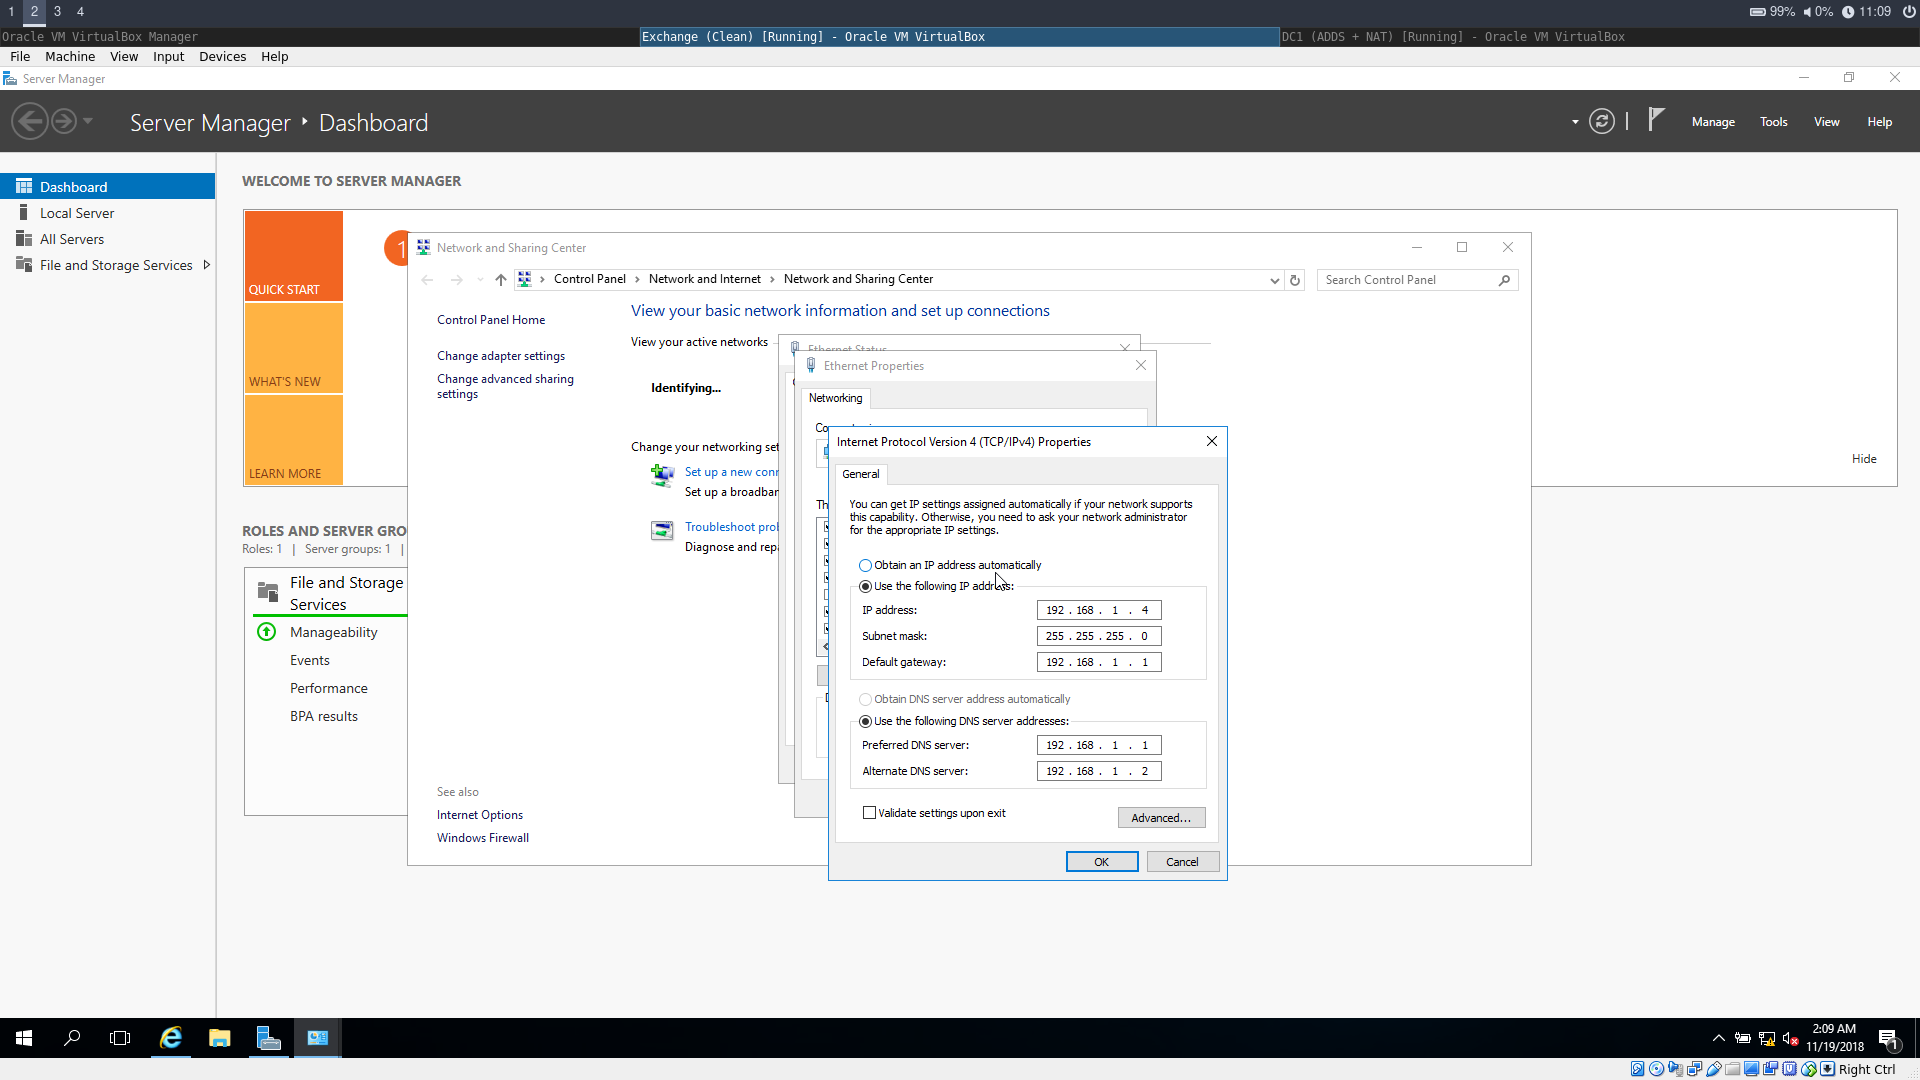
\includegraphics[width=15cm]{Pictures/Exchange/1542622148.png}
\end{center}
\subsection{Toevoegen aan het domein}
\begin{center}
	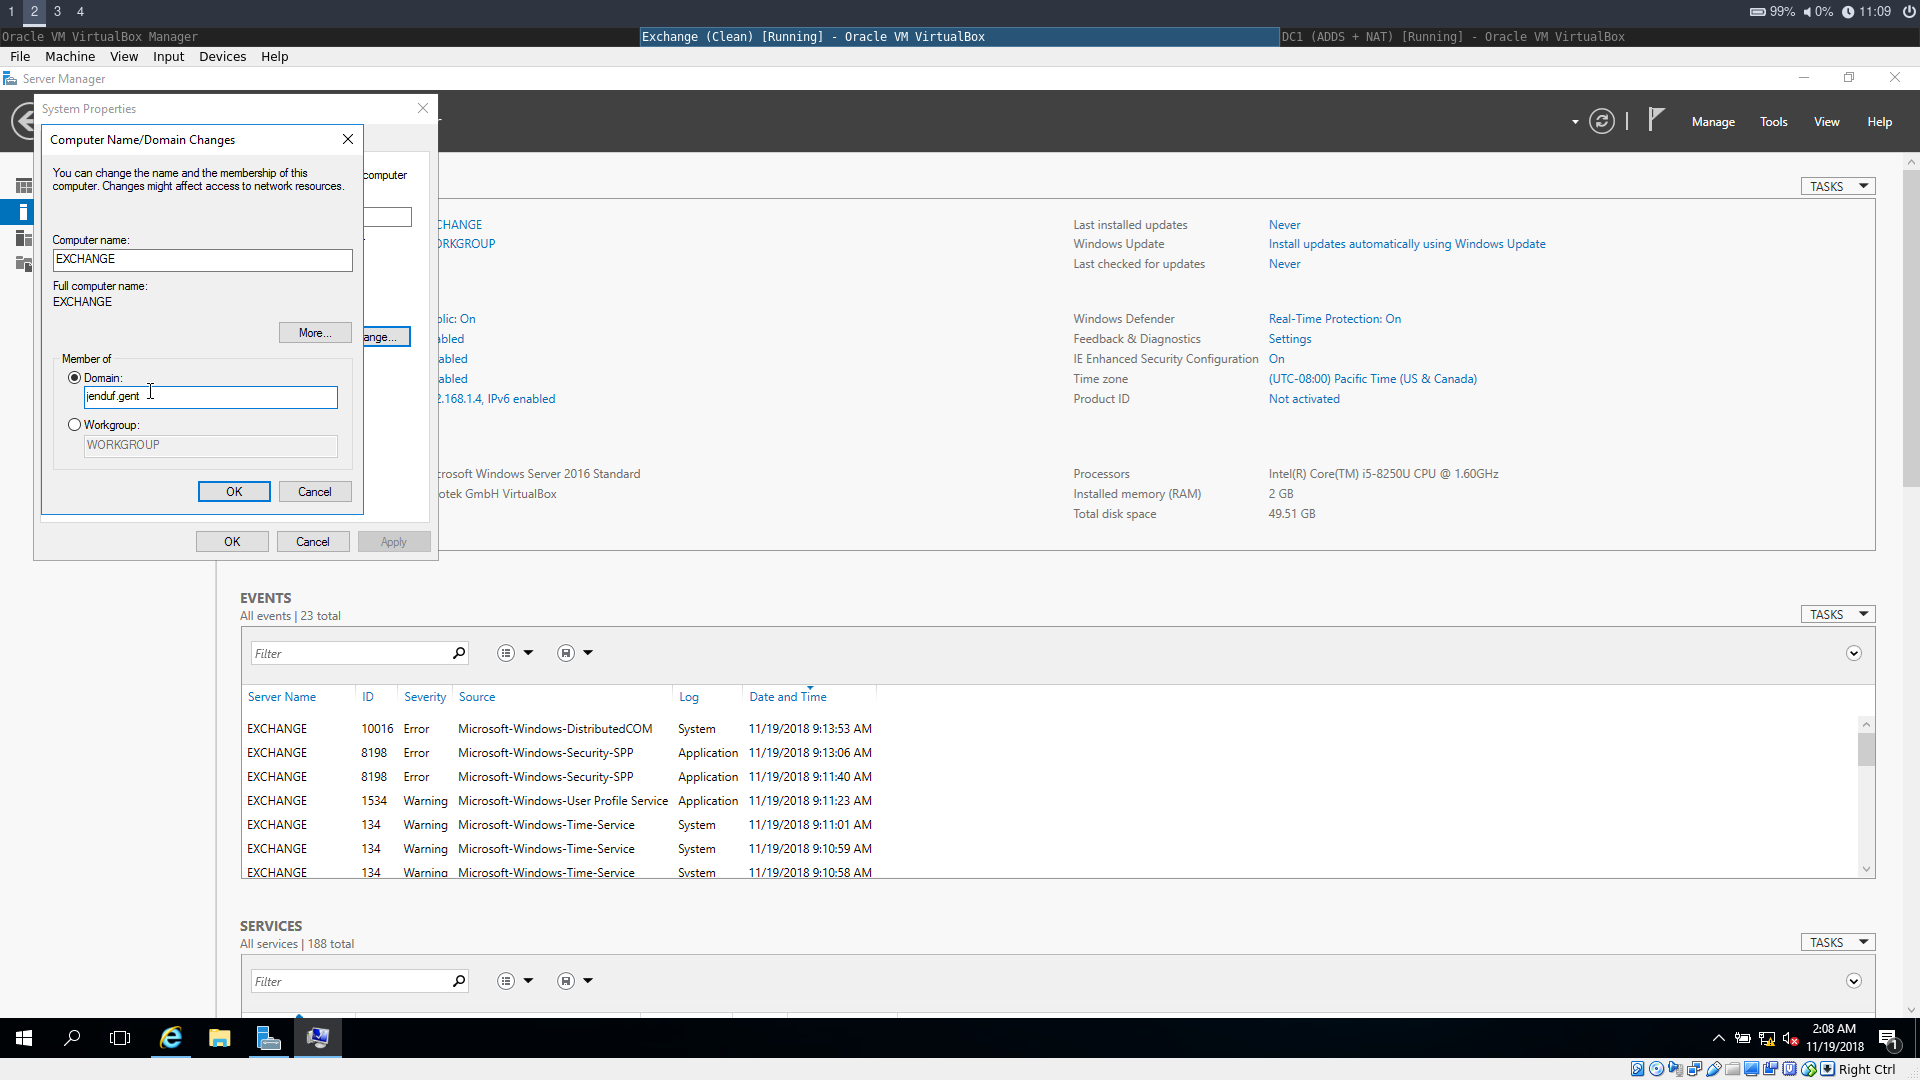
\includegraphics[width=15cm]{Pictures/Exchange/1542622164.png}
	
	Geef als domein jenduf.gent in.
\end{center}
\begin{center}
	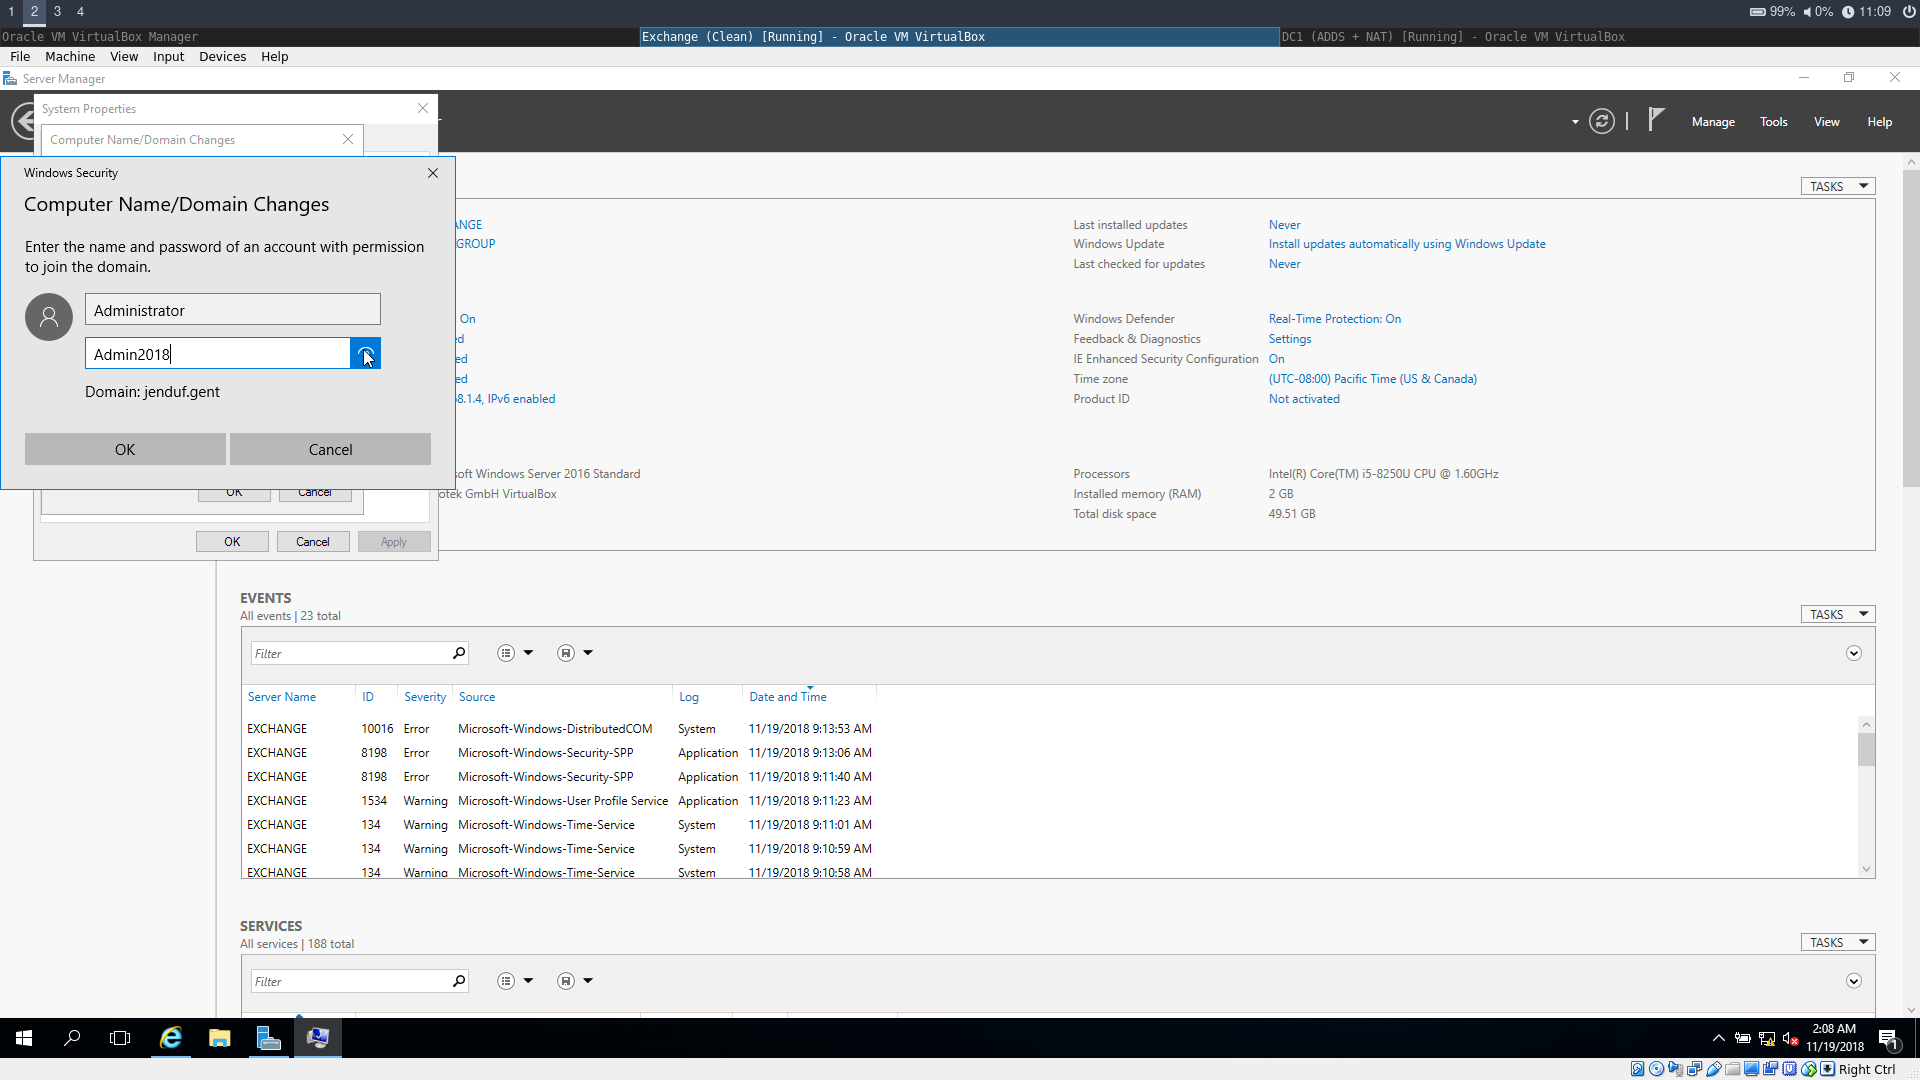
\includegraphics[width=15cm]{Pictures/Exchange/1542622176.png}
	
	Geef gebruikersnaam "Administrator" in en paswoord "Admin2018".
\end{center}
\begin{center}
	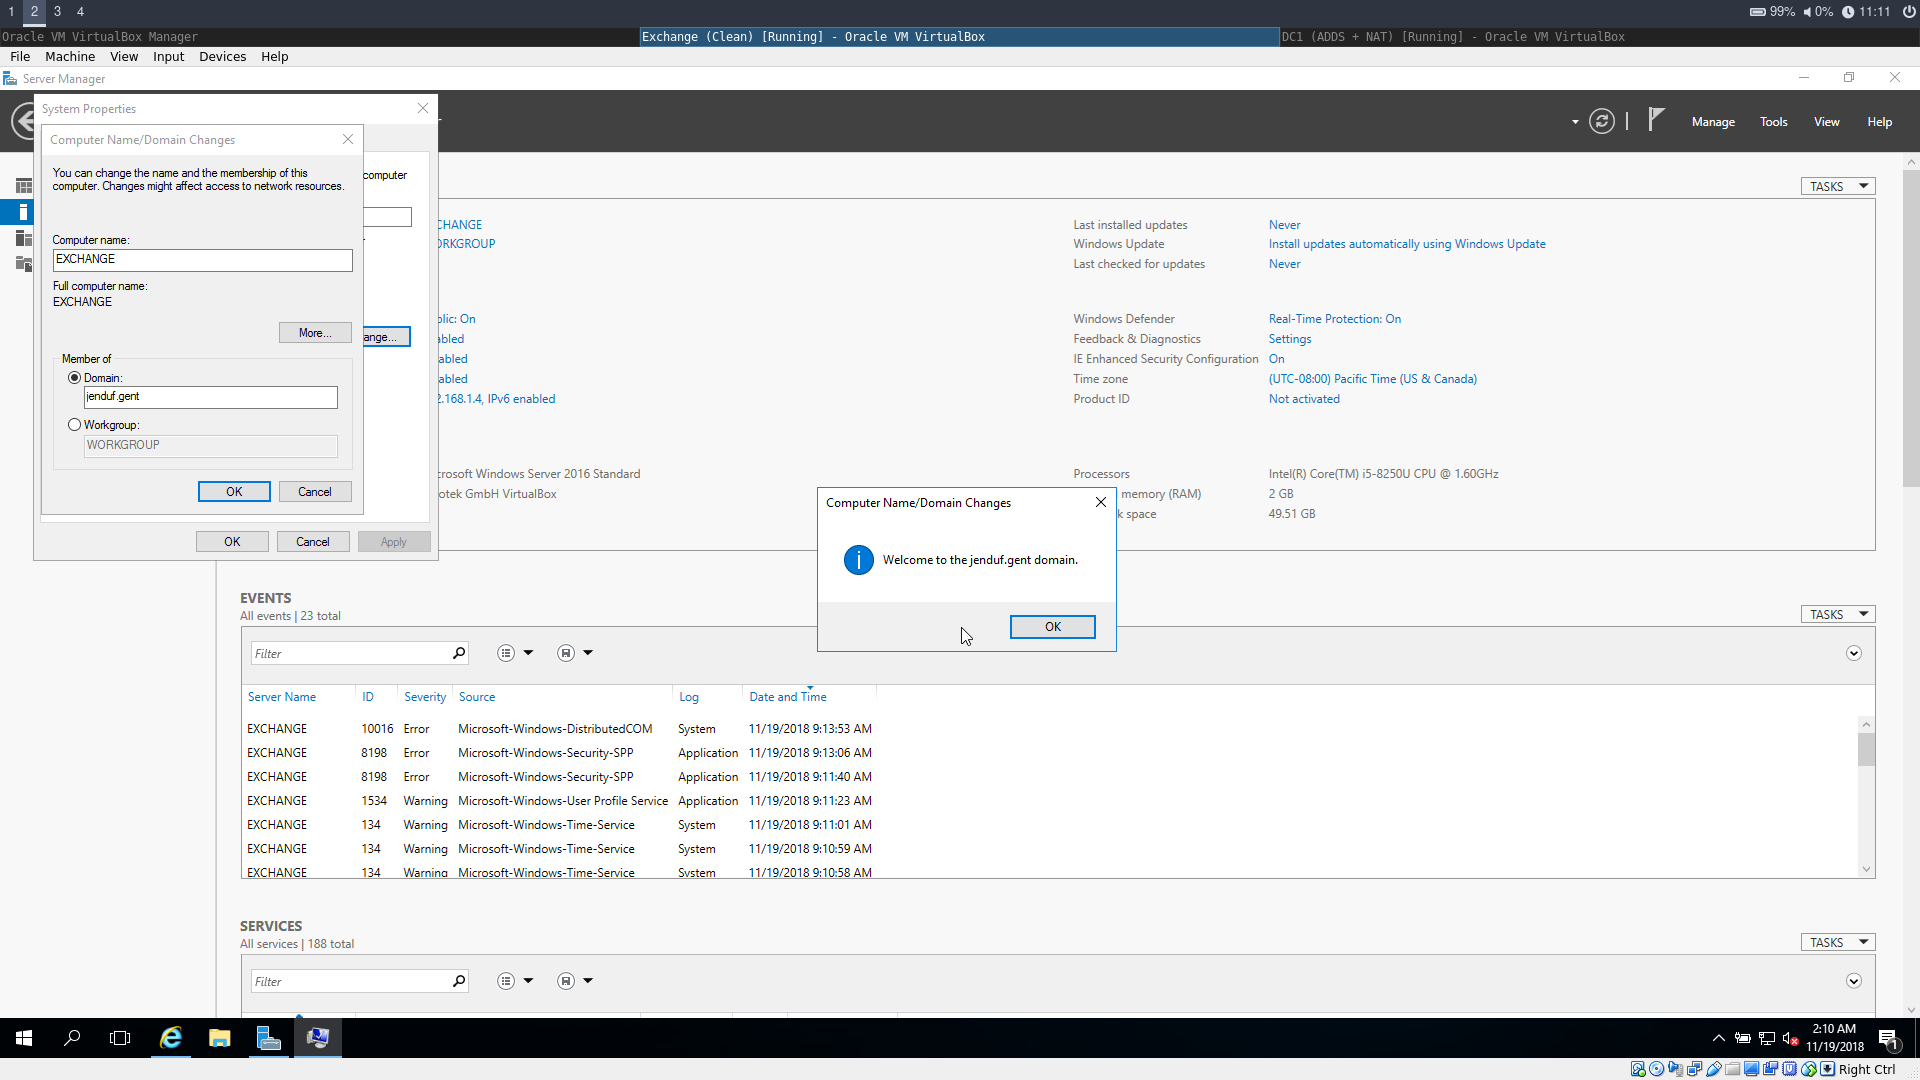
\includegraphics[width=15cm]{Pictures/Exchange/1542622272.png}
	
	De connectie is geslaagd bij het weergeven van volgende boodschap.
\end{center}

\clearpage

\section{Installatie Exchange Server}
\subsection{Prerequisites}
	\begin{center}
	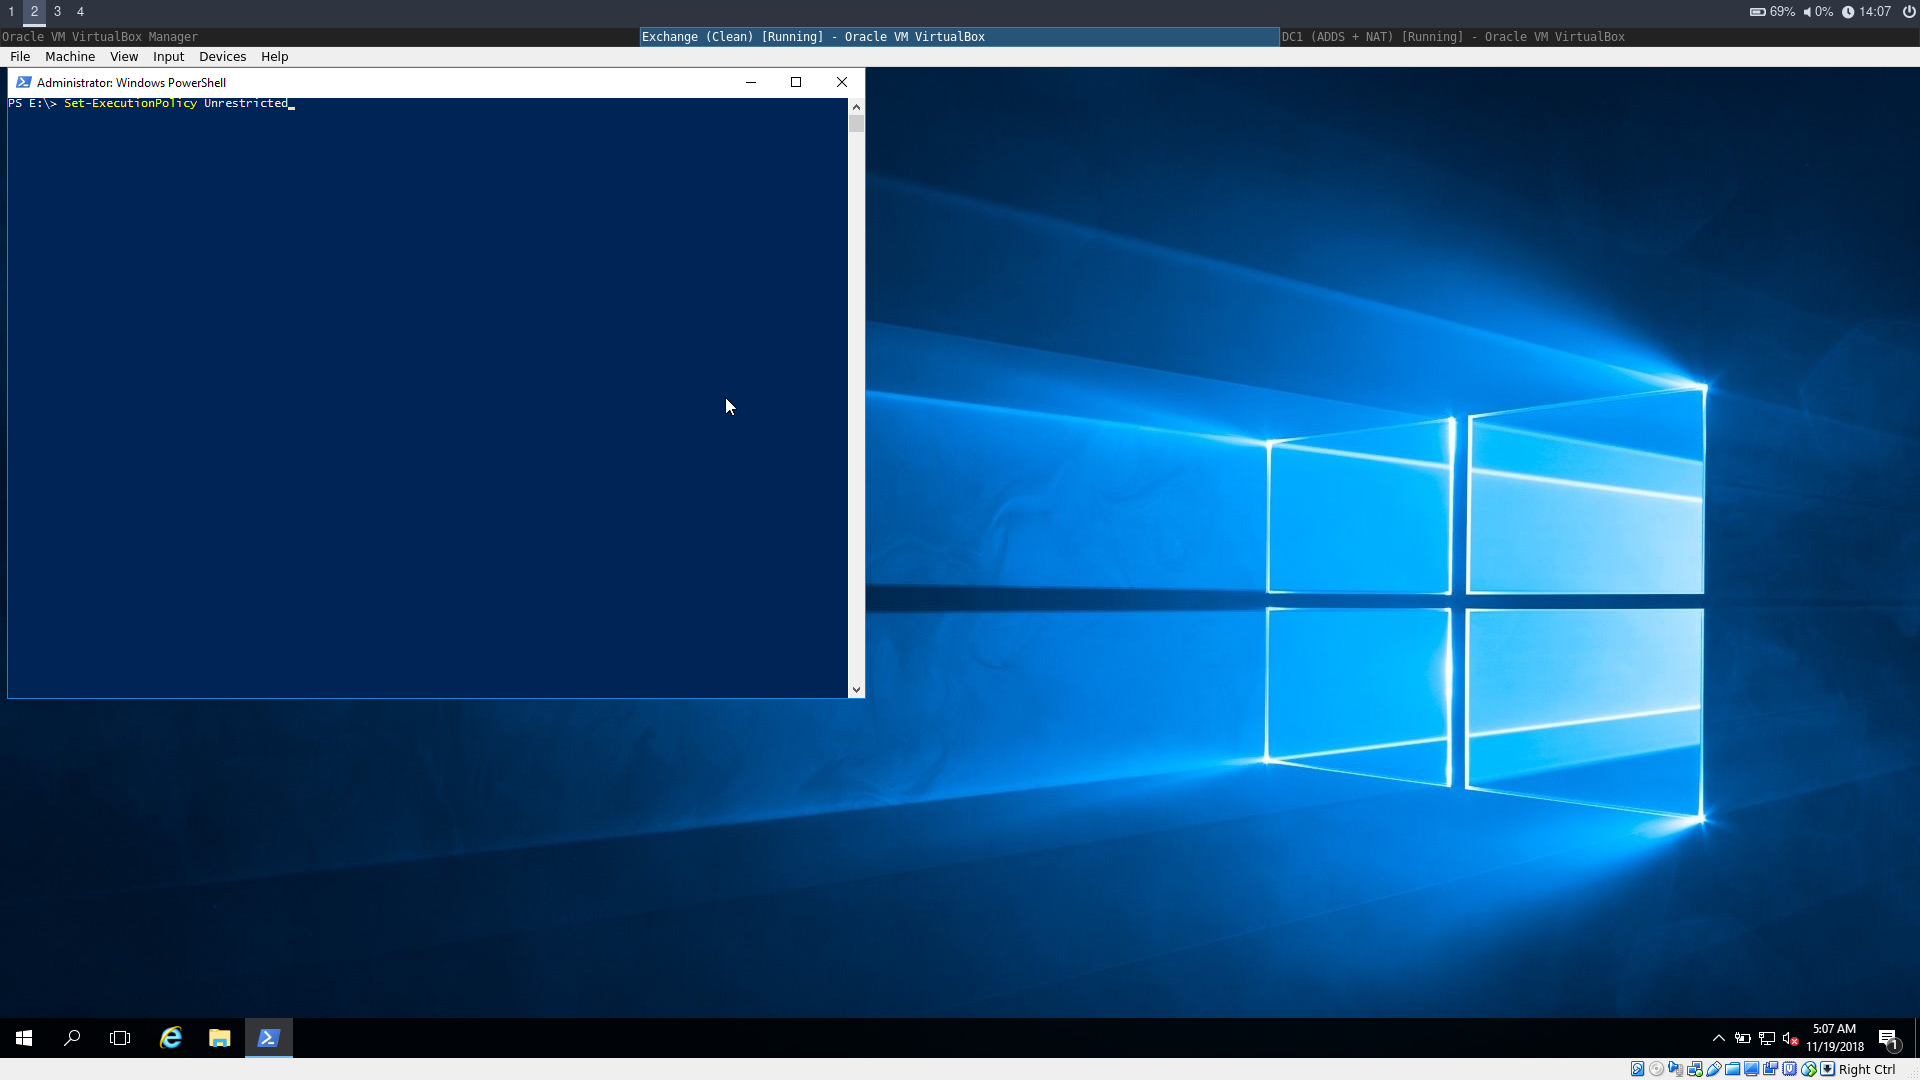
\includegraphics[width=15cm]{Pictures/Exchange/Pre/1542632844.png}
	
	Stel het "ExecutionPolicy" op "Unrestricted".
\end{center}
	\begin{center}
	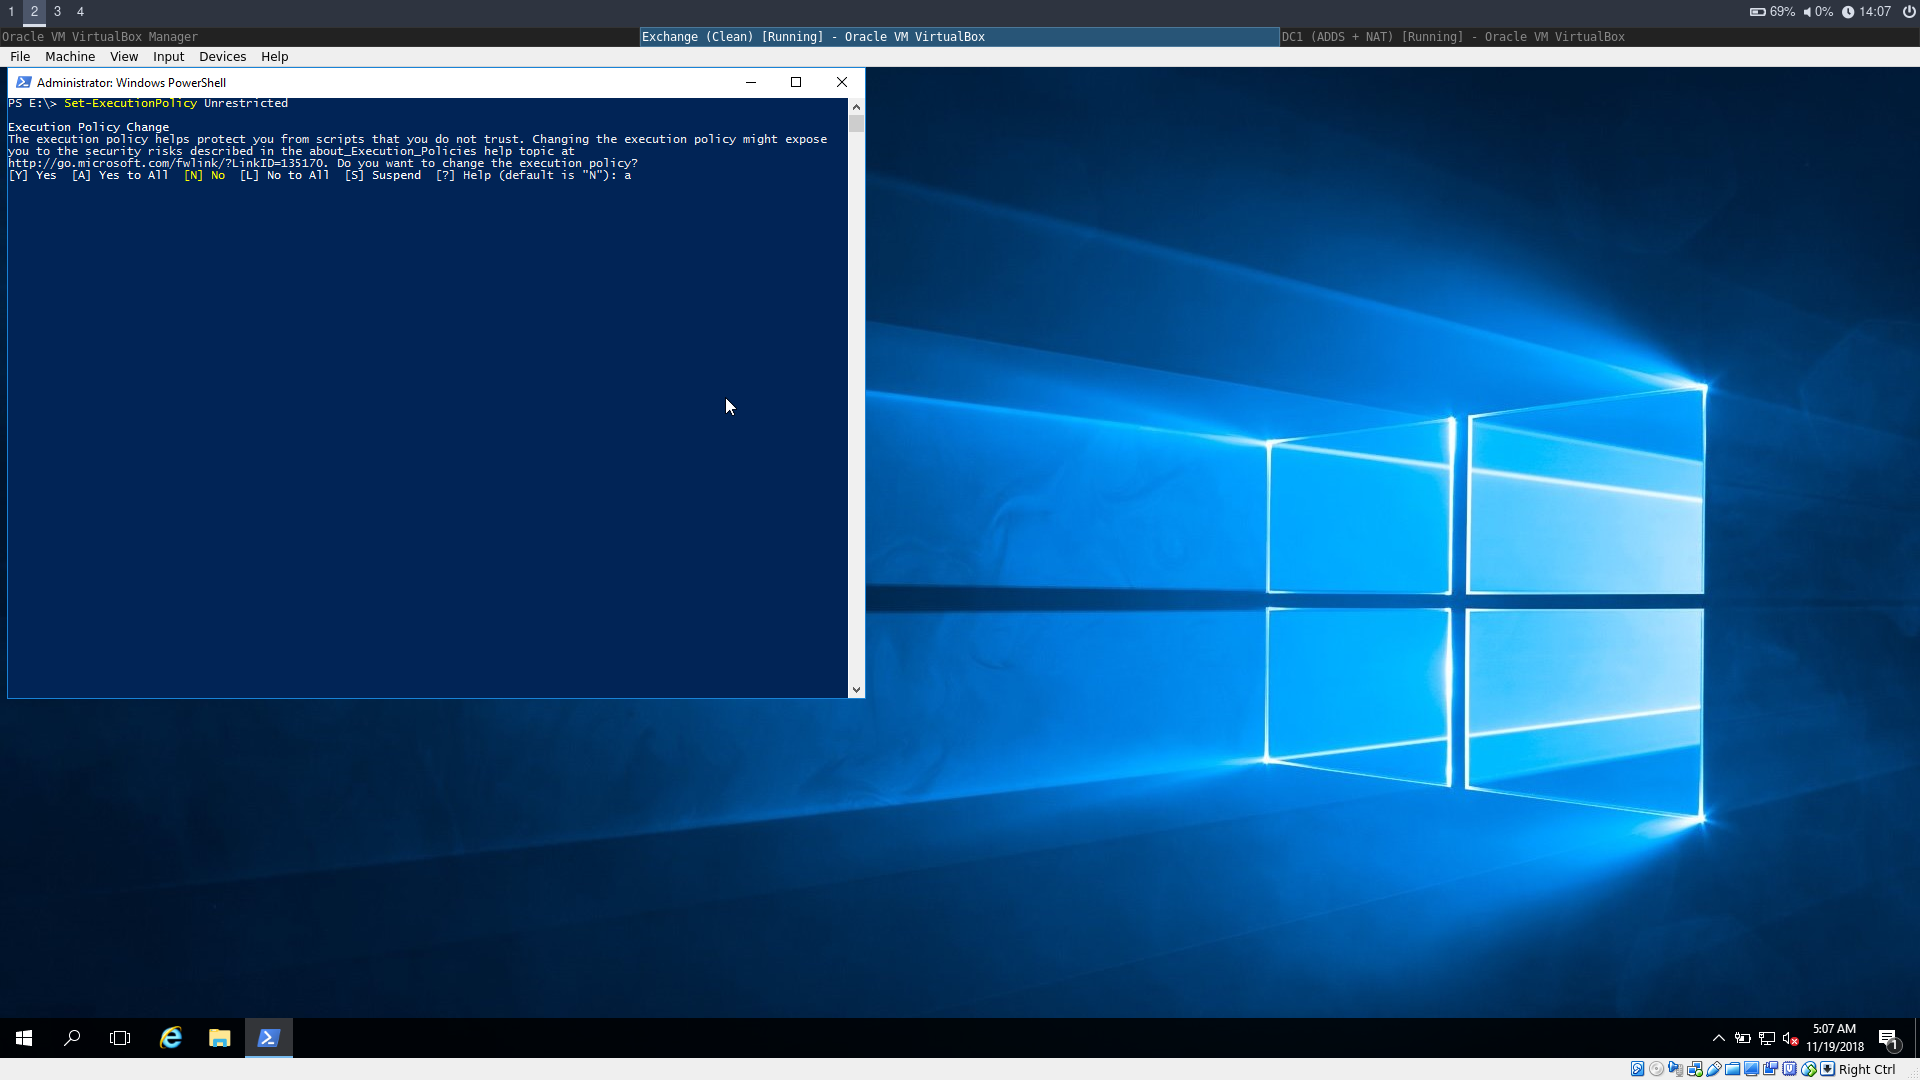
\includegraphics[width=15cm]{Pictures/Exchange/Pre/1542632849.png}
	
	Selecteer "Yes to All".
\end{center}
	\begin{center}
	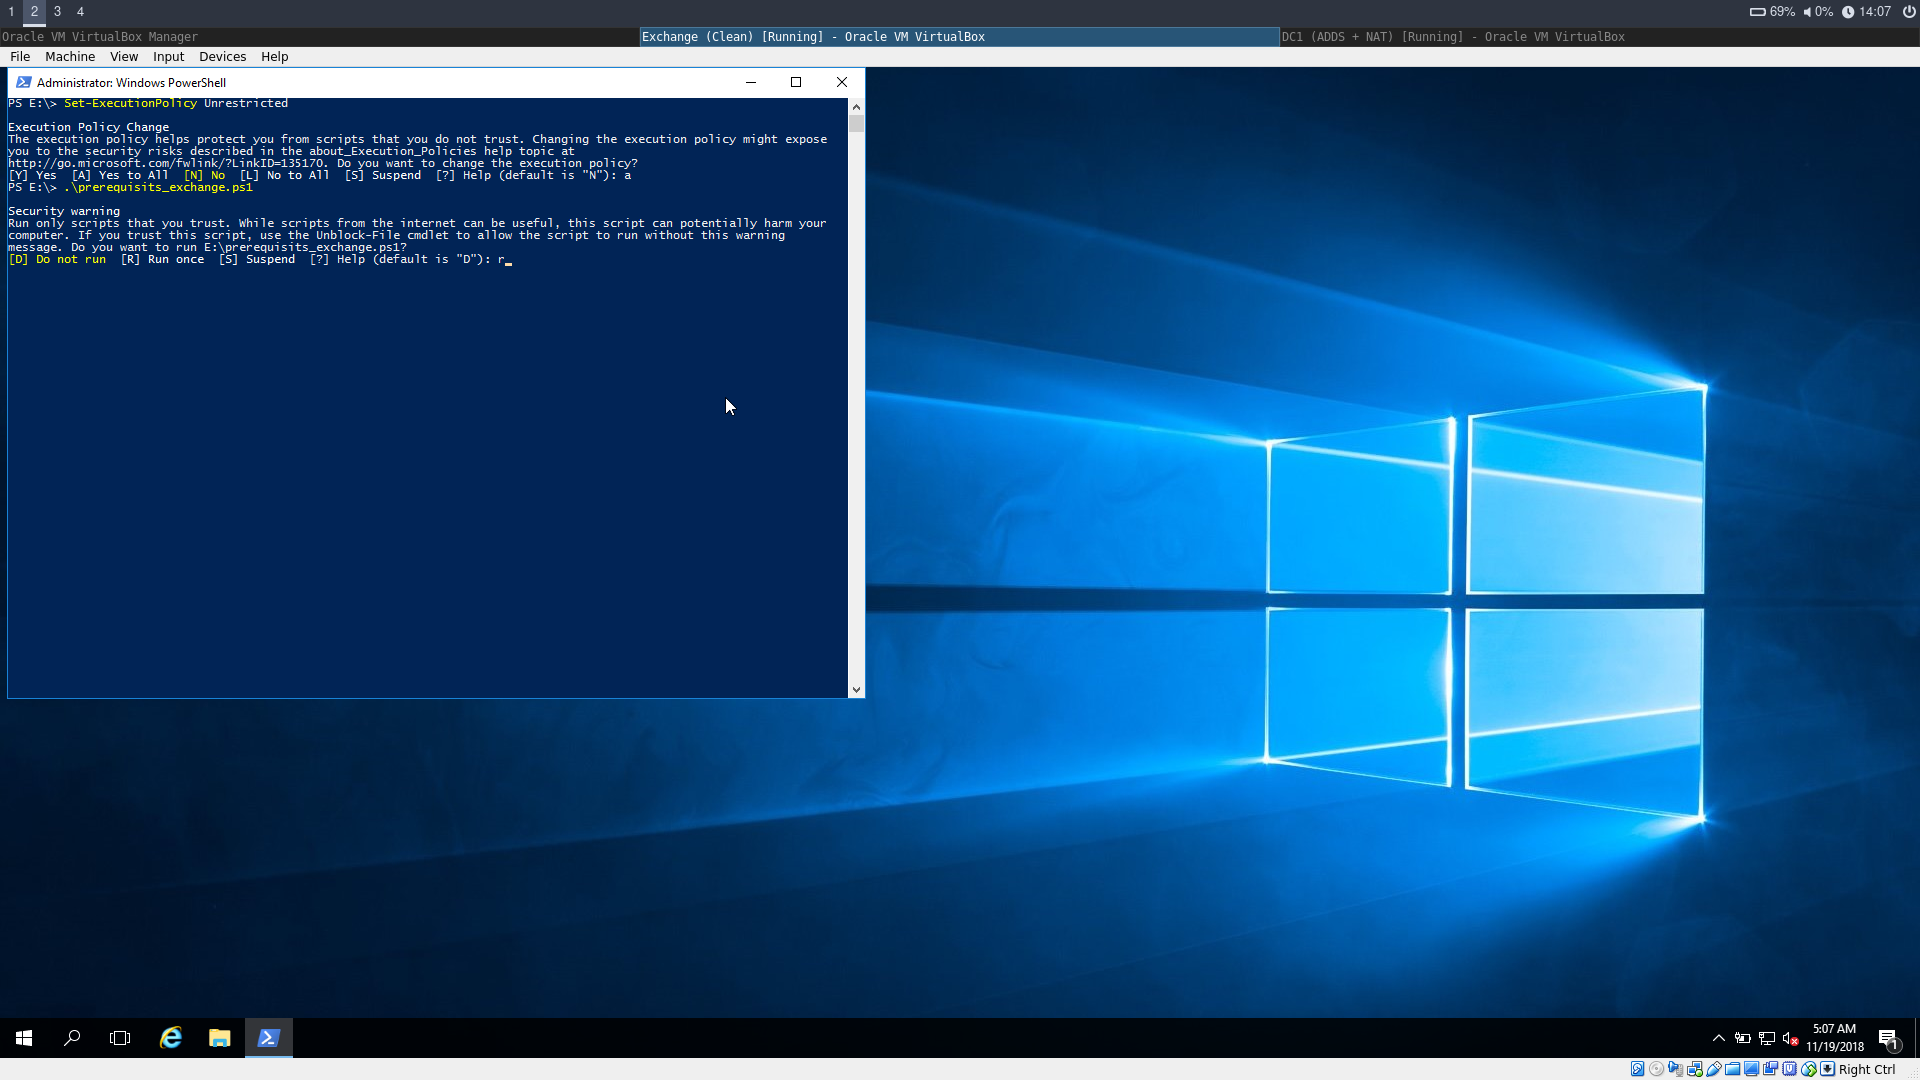
\includegraphics[width=15cm]{Pictures/Exchange/Pre/1542632856.png}
	
	Voer het script uit en selecteer "Run once".
\end{center}
	\begin{center}
	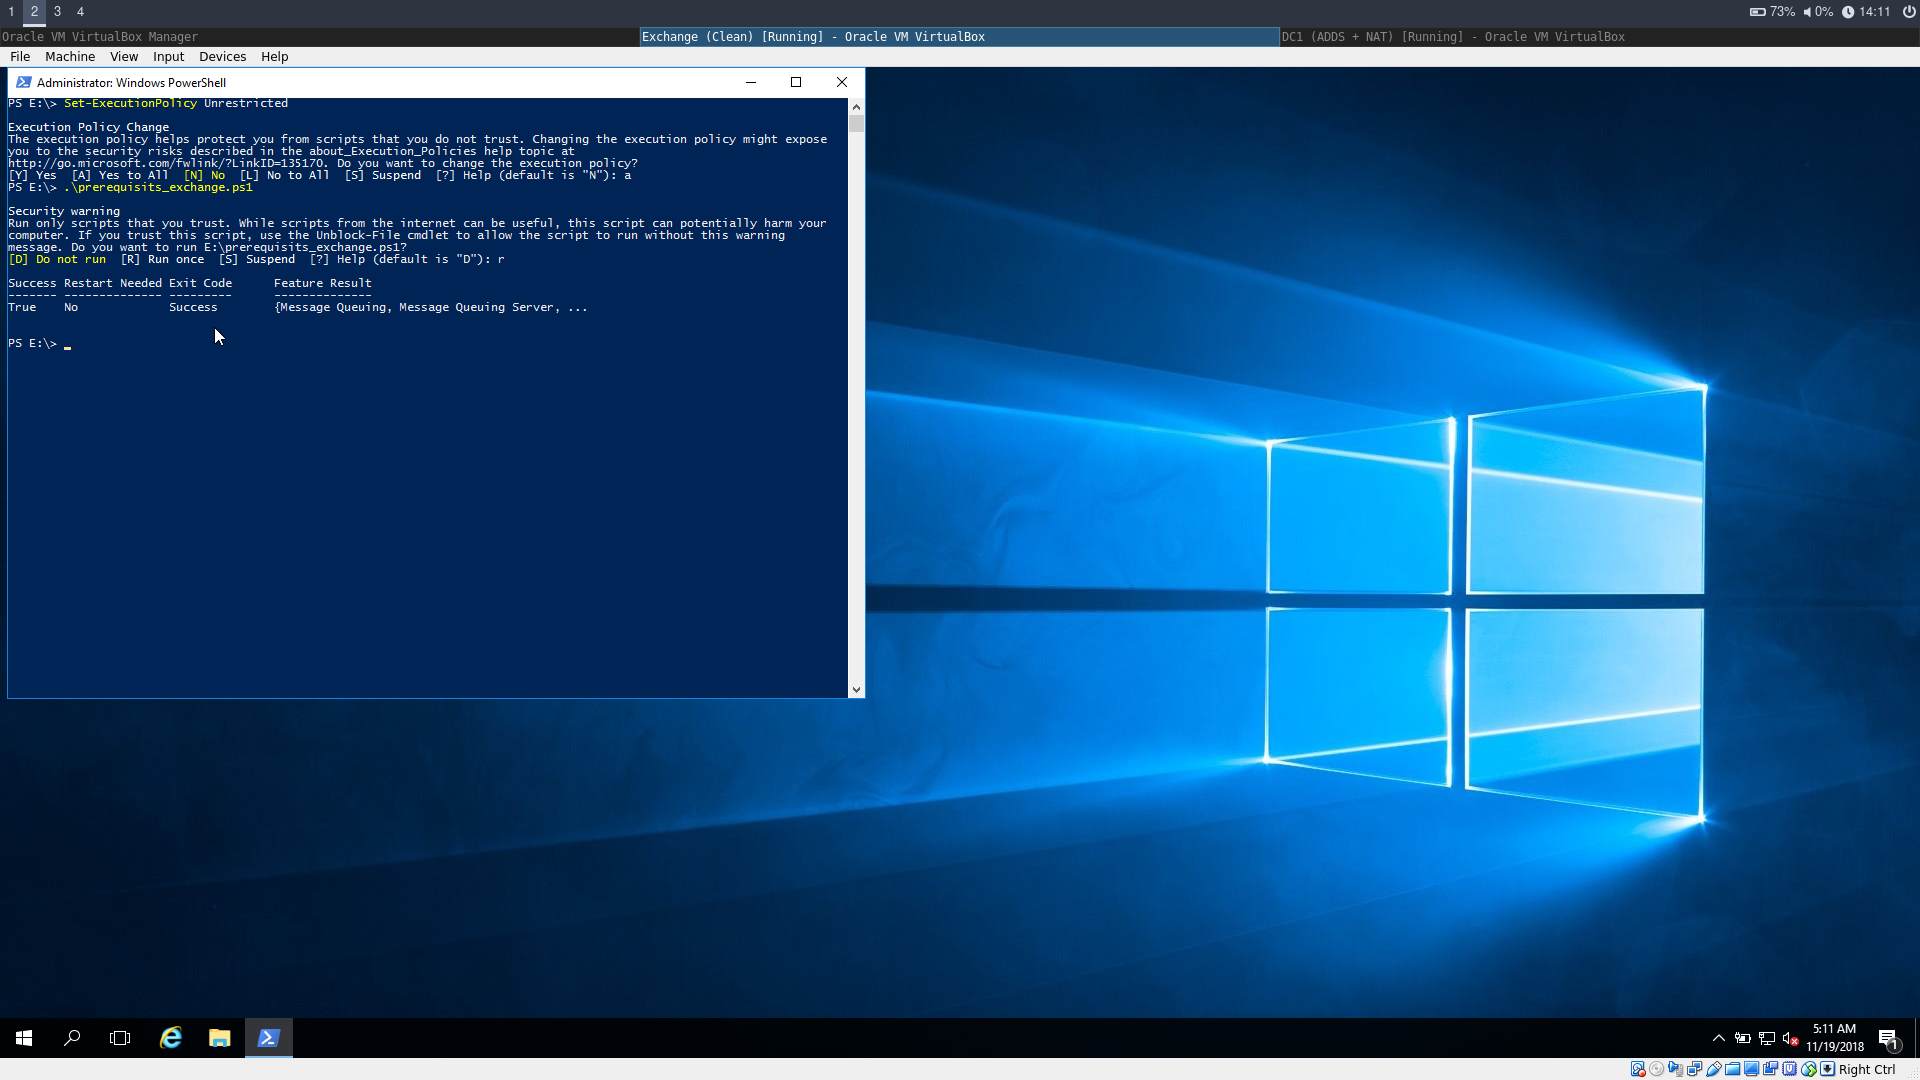
\includegraphics[width=15cm]{Pictures/Exchange/Pre/1542633119.png}
\end{center}
	\begin{center}
	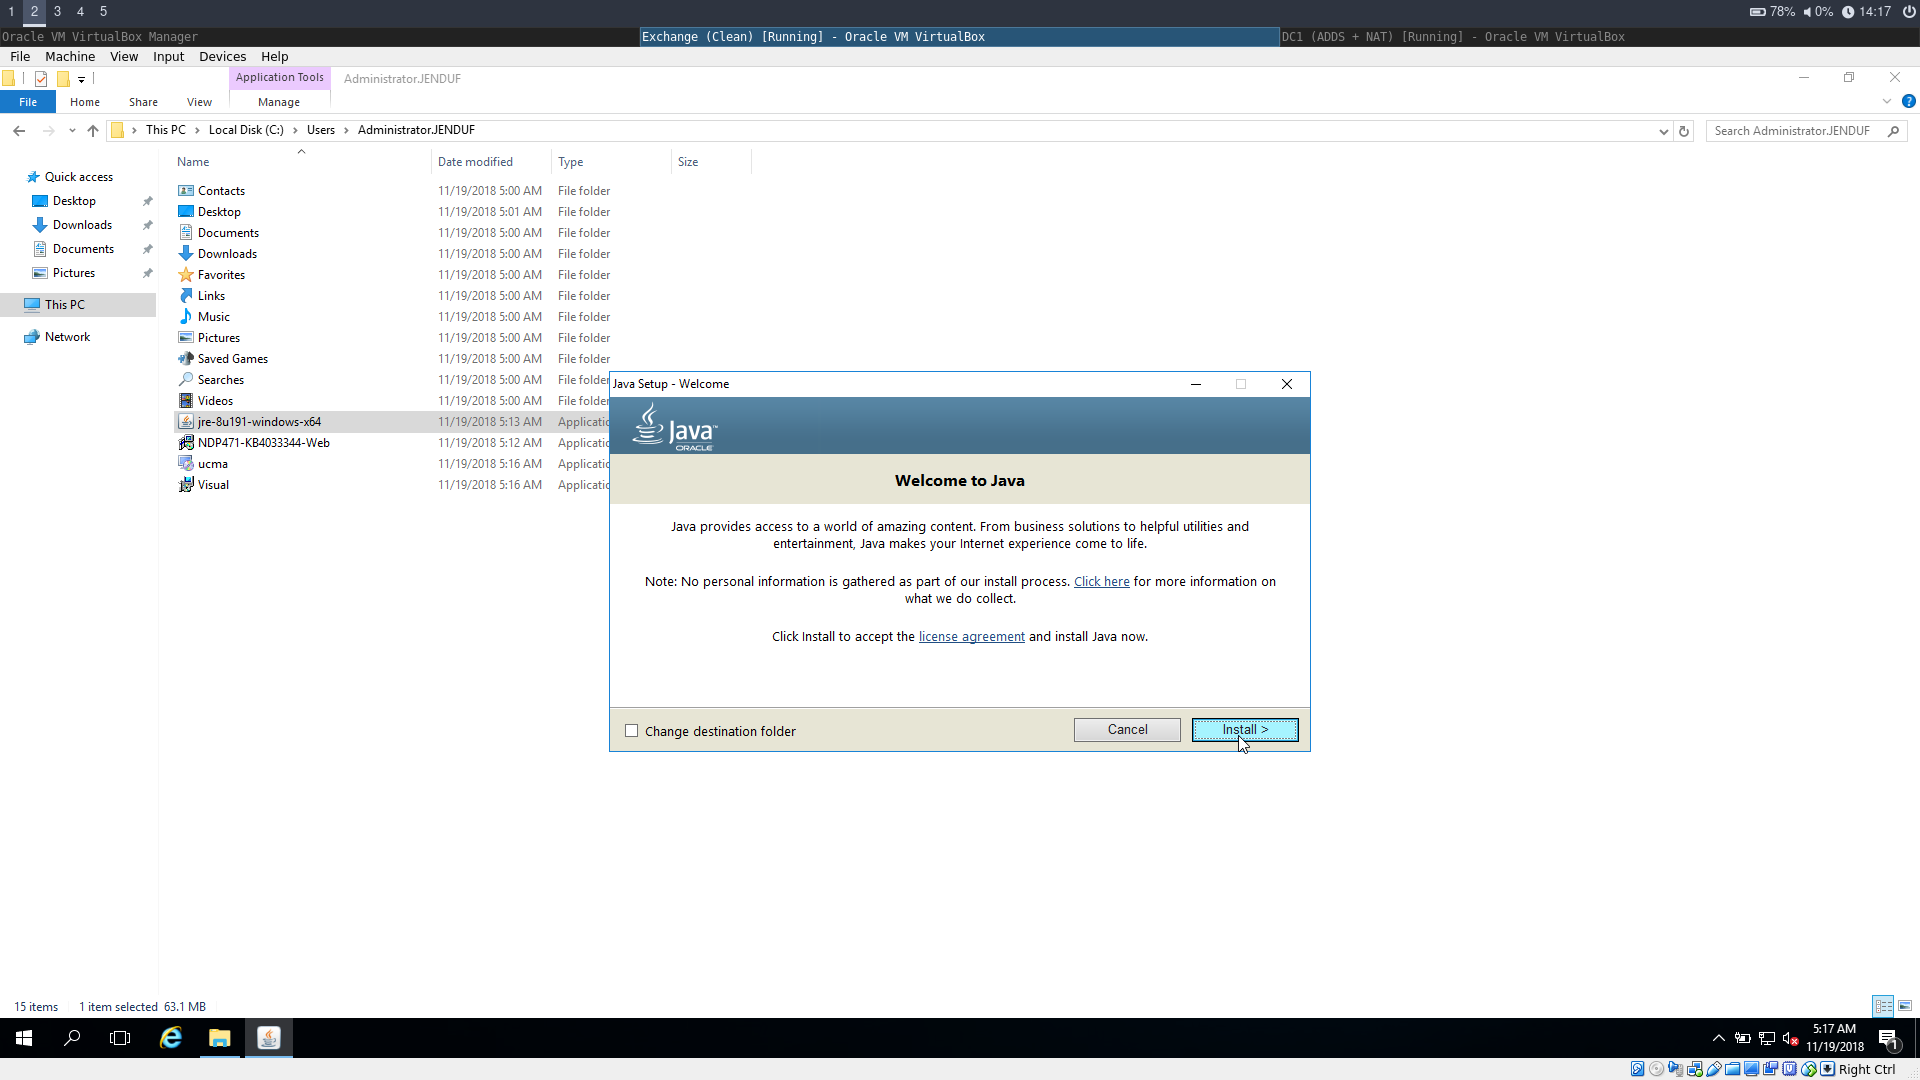
\includegraphics[width=15cm]{Pictures/Exchange/Pre/1542633454.png}
	
	Installeer Java.
\end{center}
	\begin{center}
	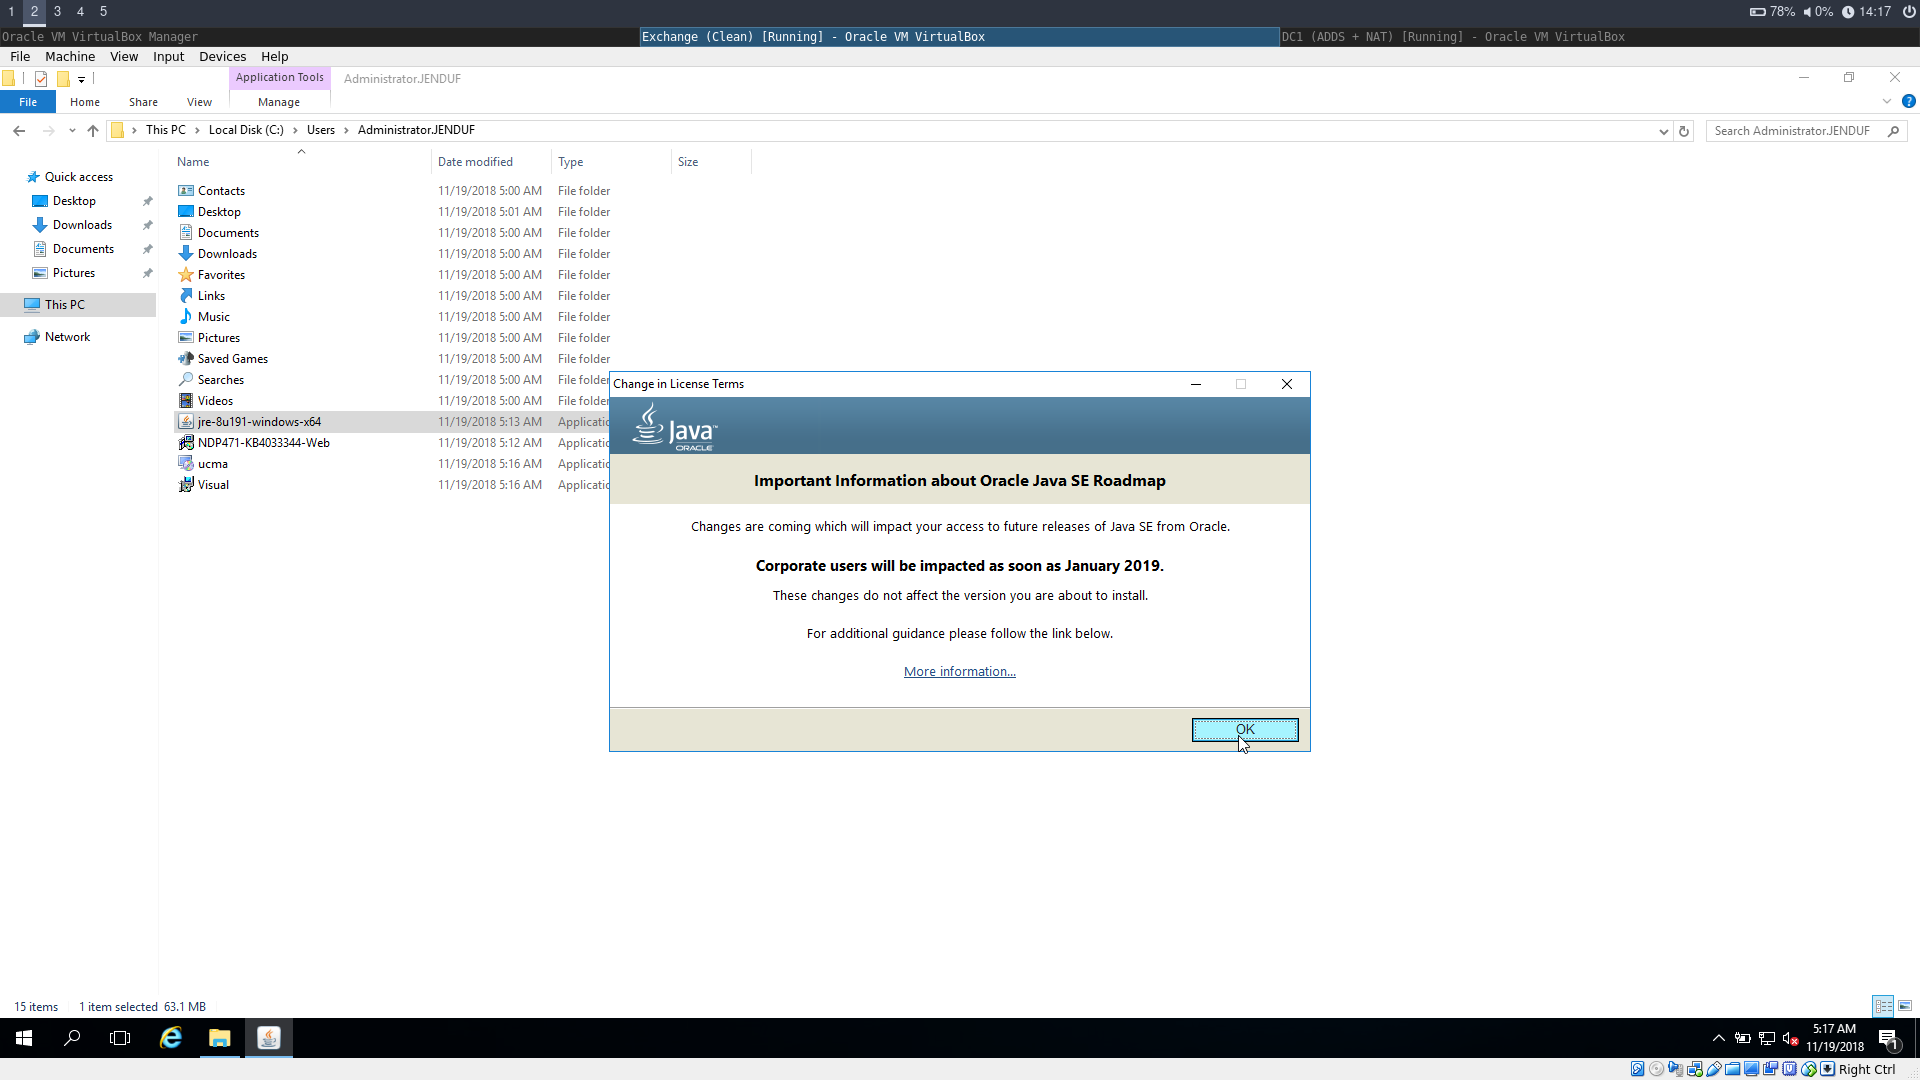
\includegraphics[width=15cm]{Pictures/Exchange/Pre/1542633458.png}
\end{center}
	\begin{center}
	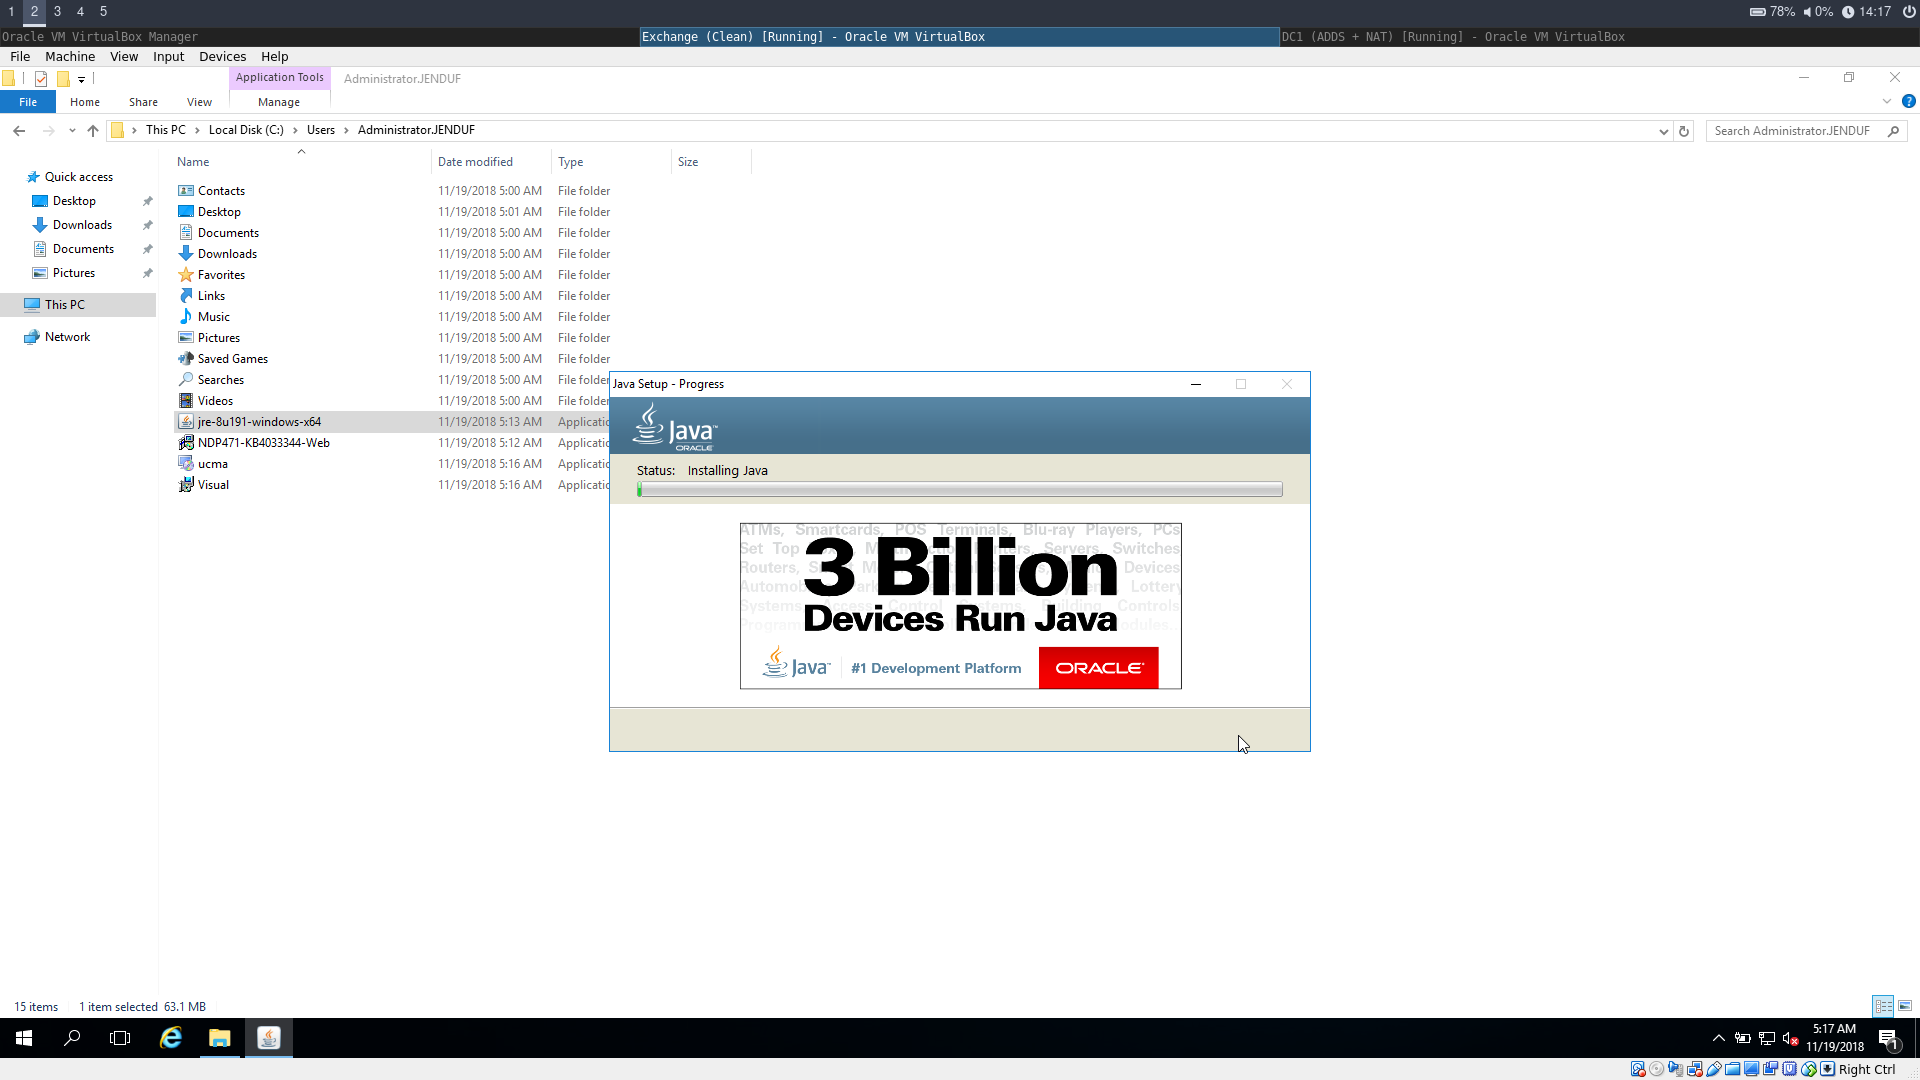
\includegraphics[width=15cm]{Pictures/Exchange/Pre/1542633460.png}
\end{center}
	\begin{center}
	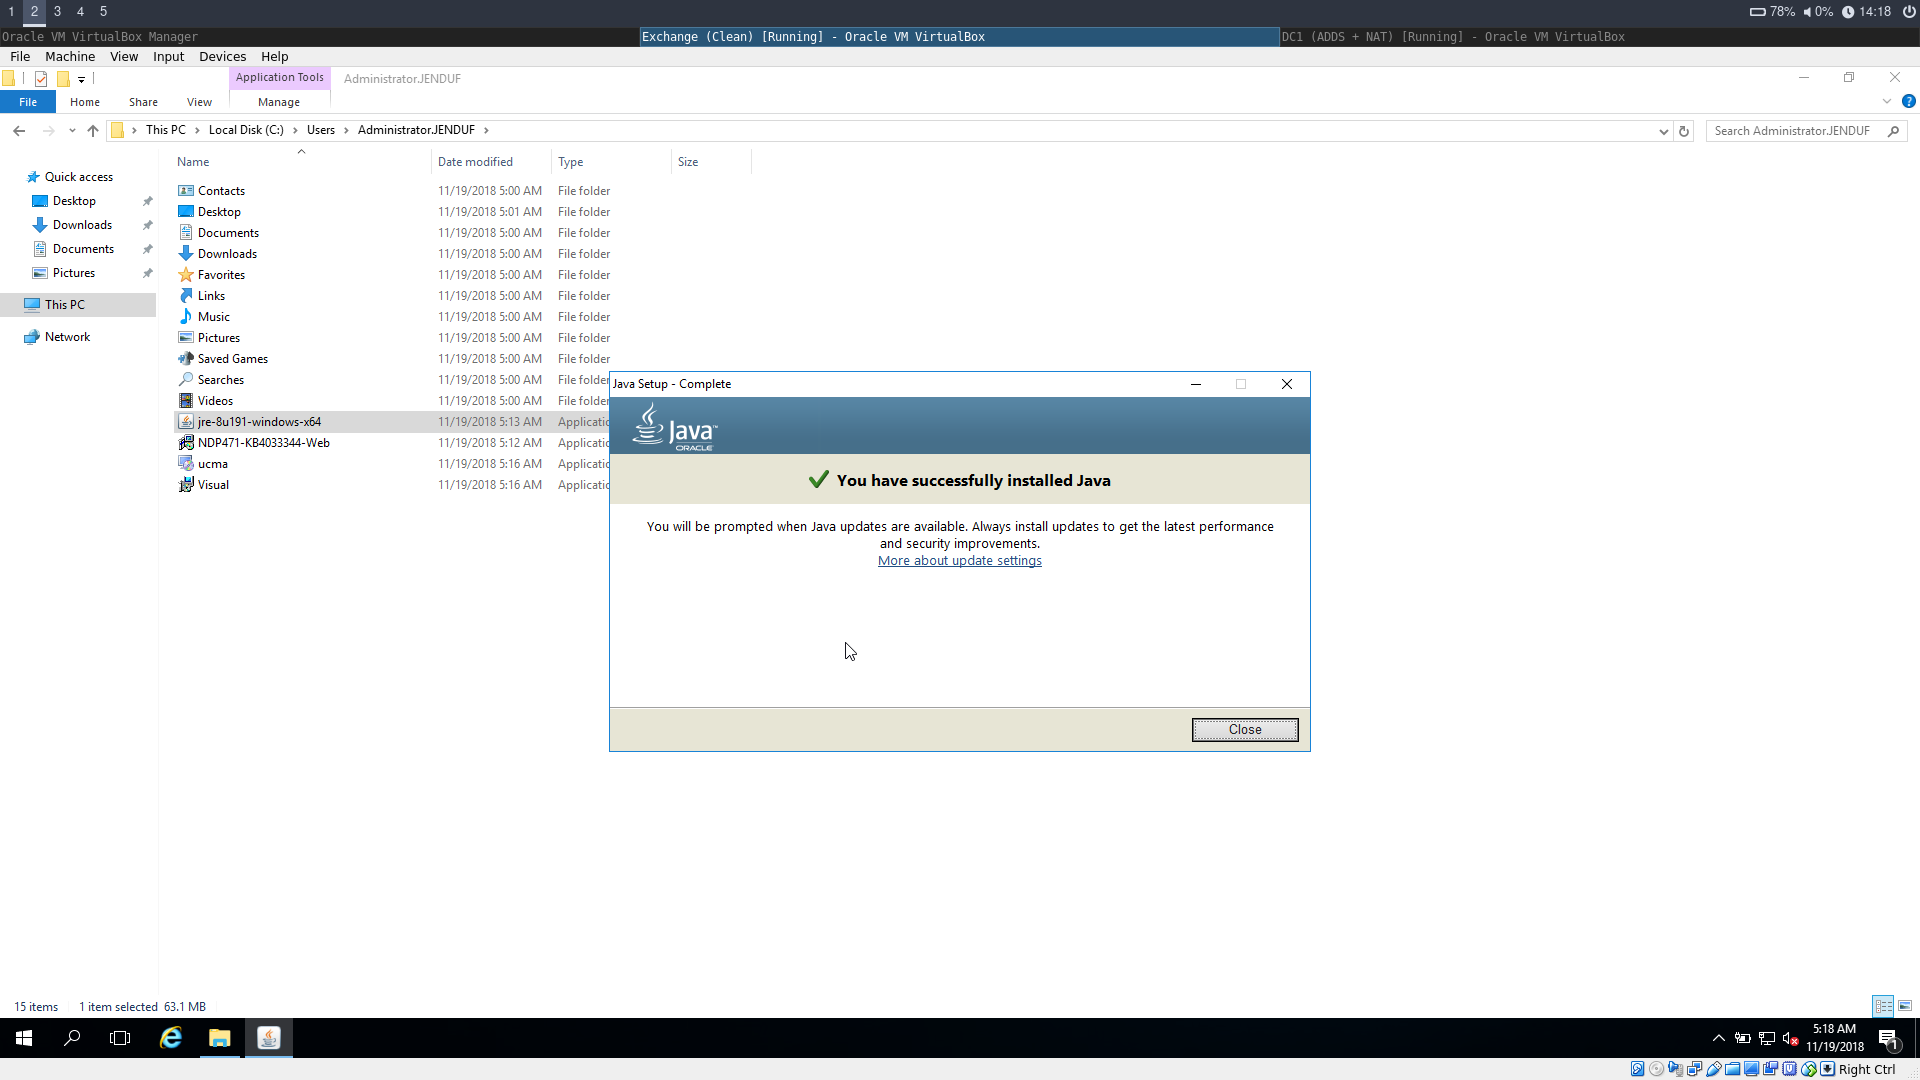
\includegraphics[width=15cm]{Pictures/Exchange/Pre/1542633487.png}
\end{center}
	\begin{center}
	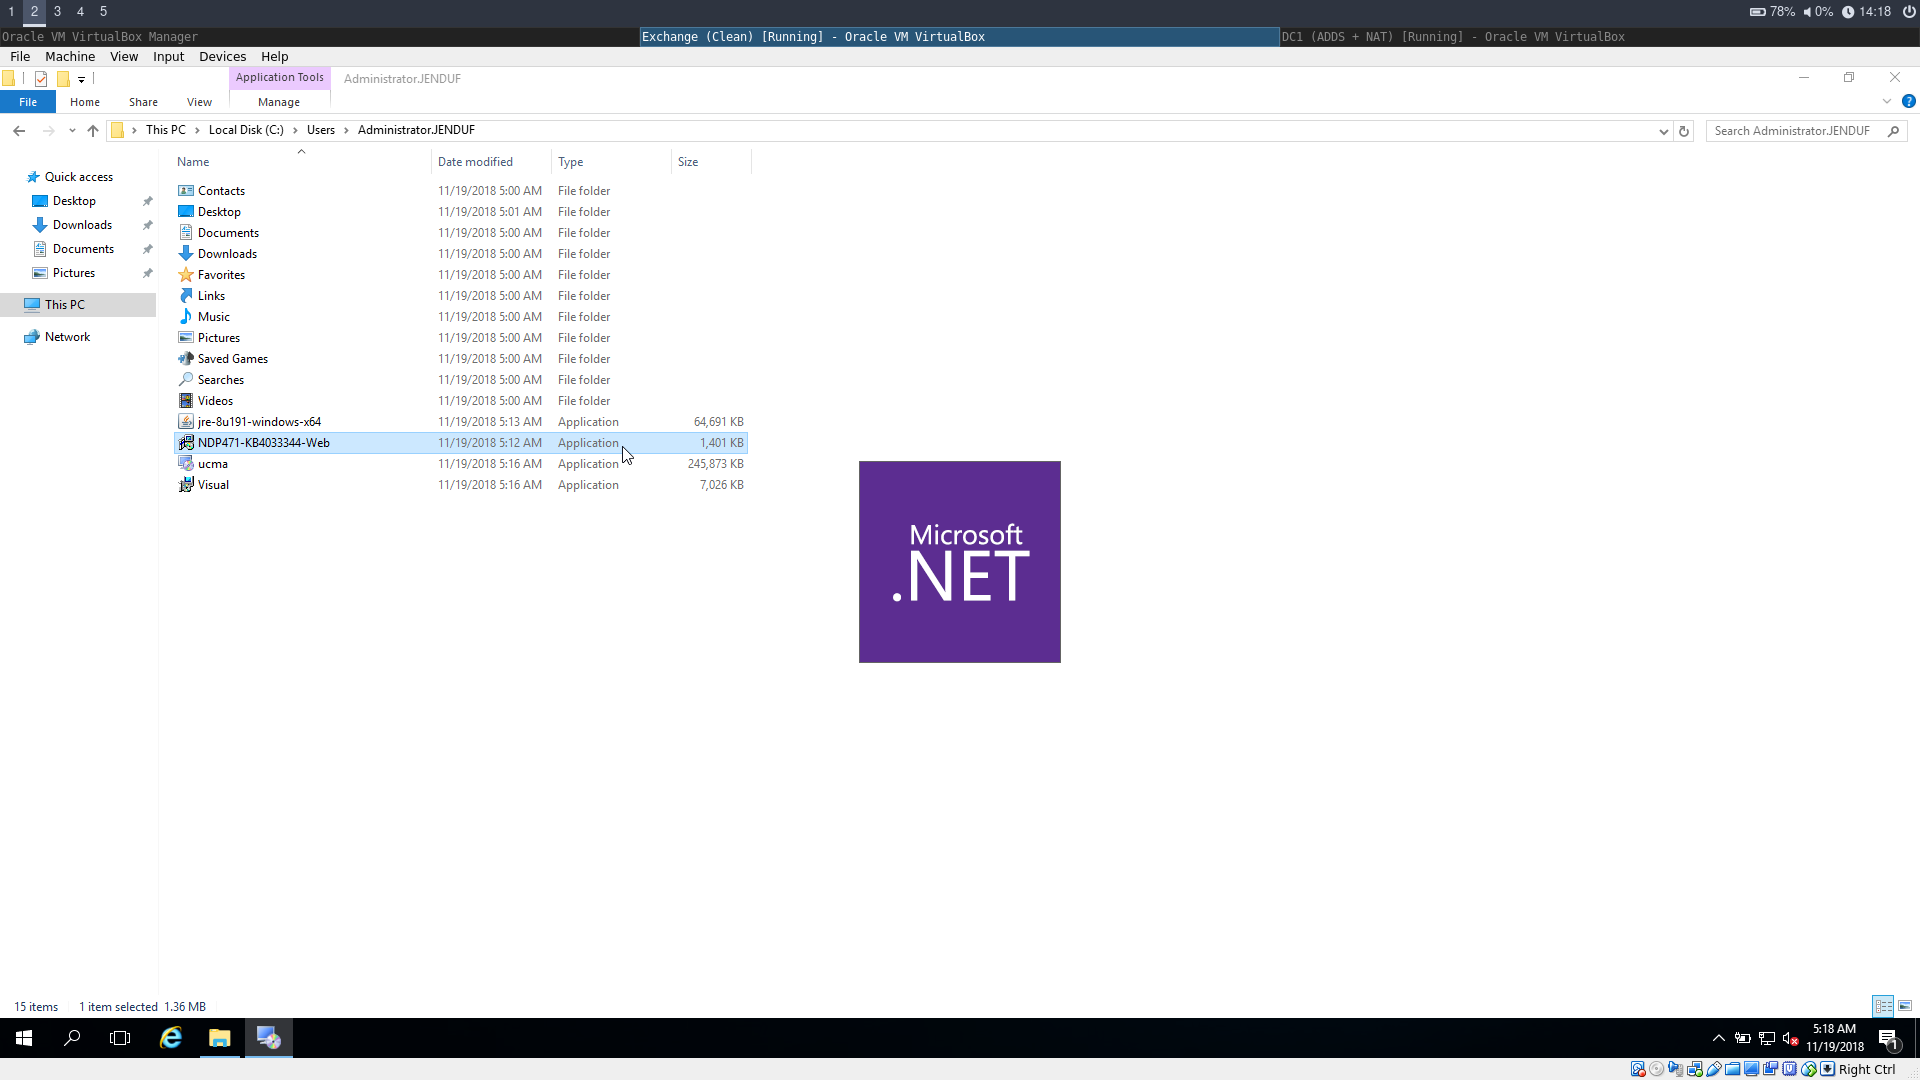
\includegraphics[width=15cm]{Pictures/Exchange/Pre/1542633495.png}
\end{center}
	\begin{center}
	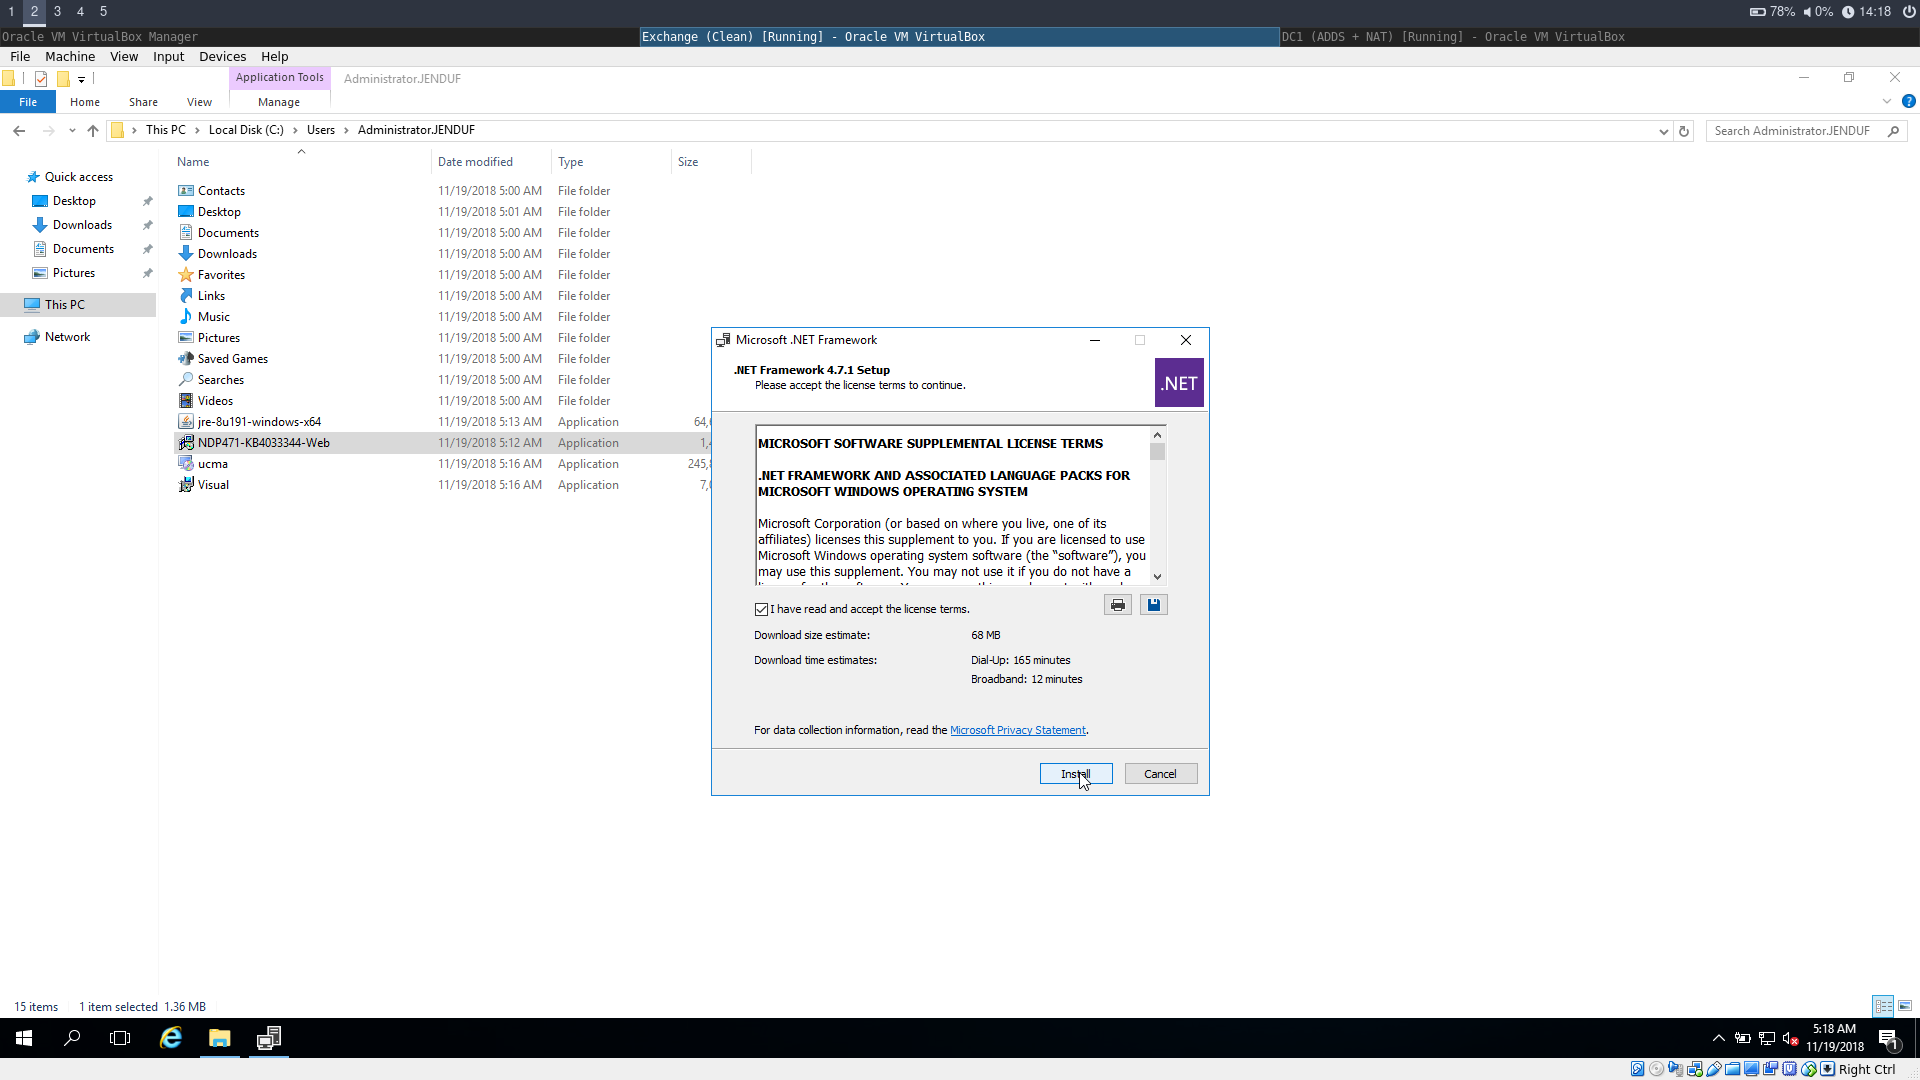
\includegraphics[width=15cm]{Pictures/Exchange/Pre/1542633503.png}
	
		Ga akkoord met de voorwaarden en druk op "Install".
\end{center}
	\begin{center}
	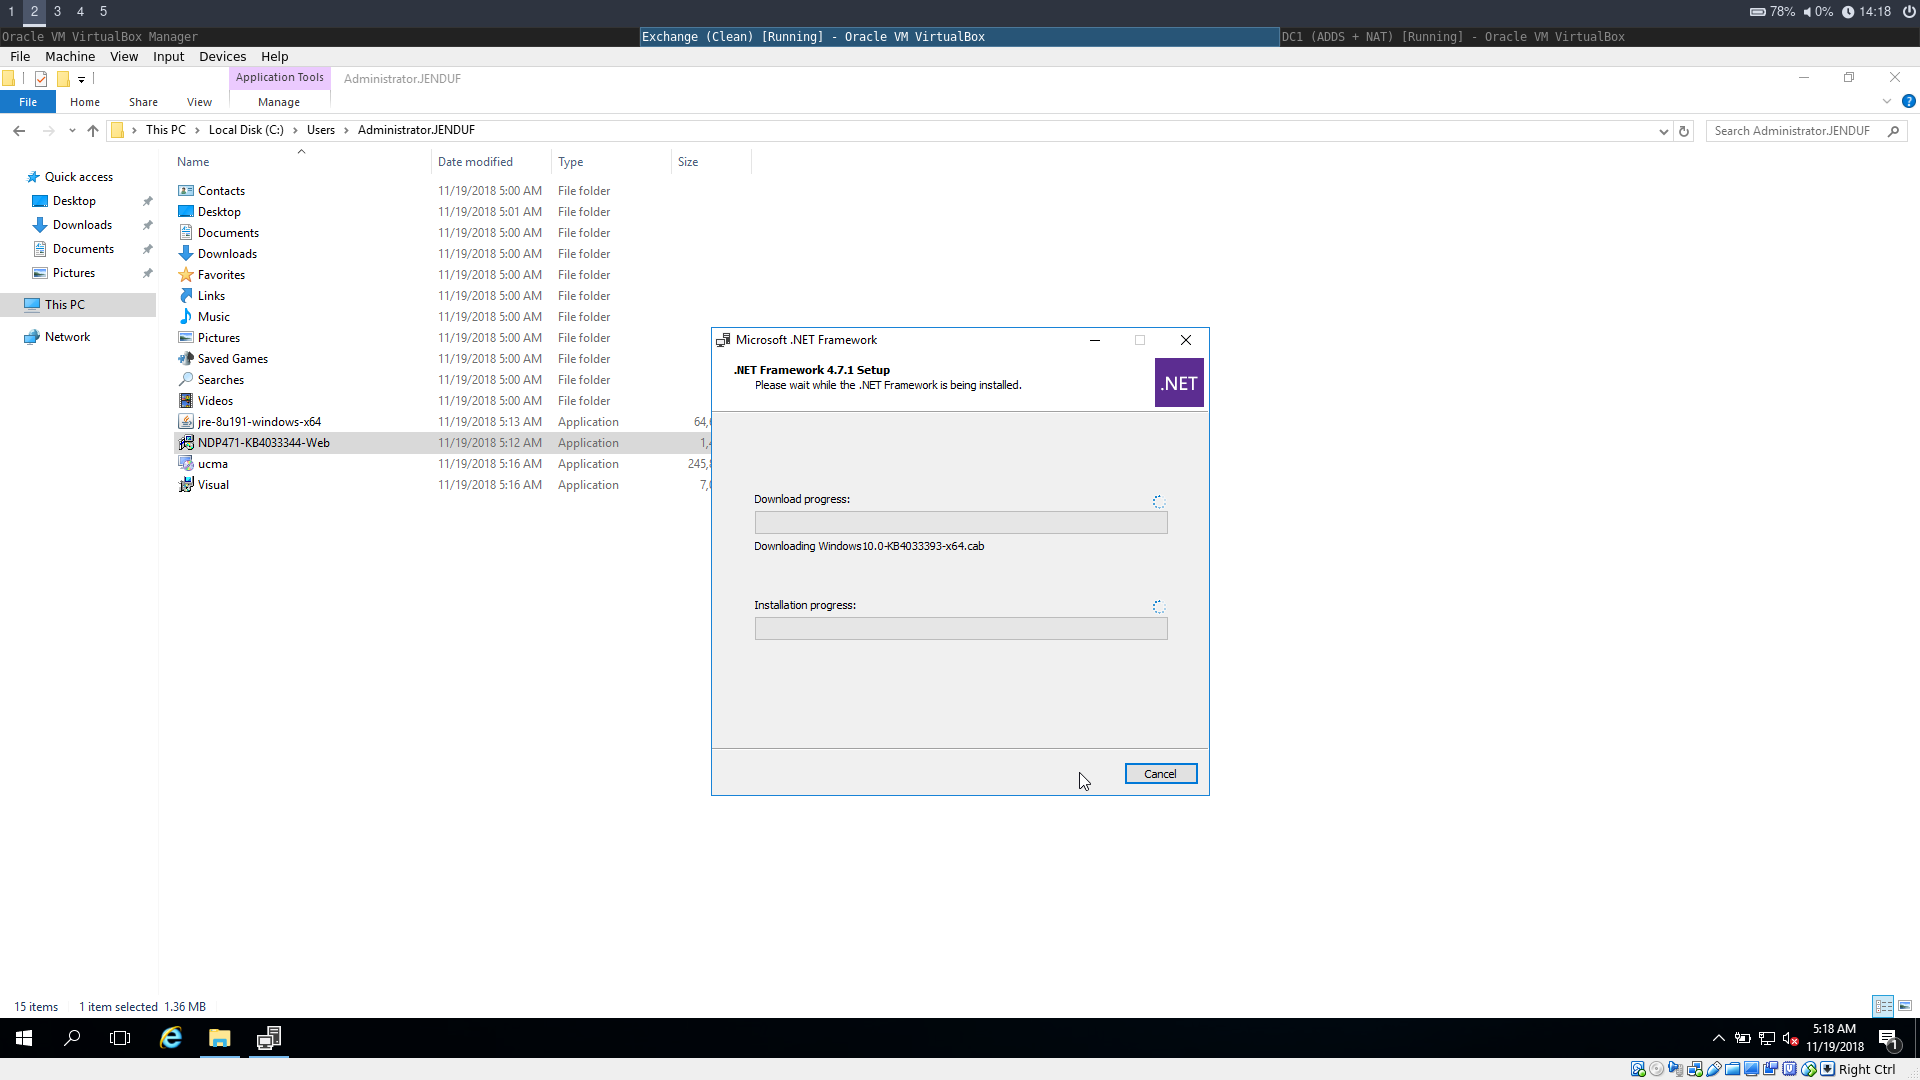
\includegraphics[width=15cm]{Pictures/Exchange/Pre/1542633506.png}
\end{center}
	\begin{center}
	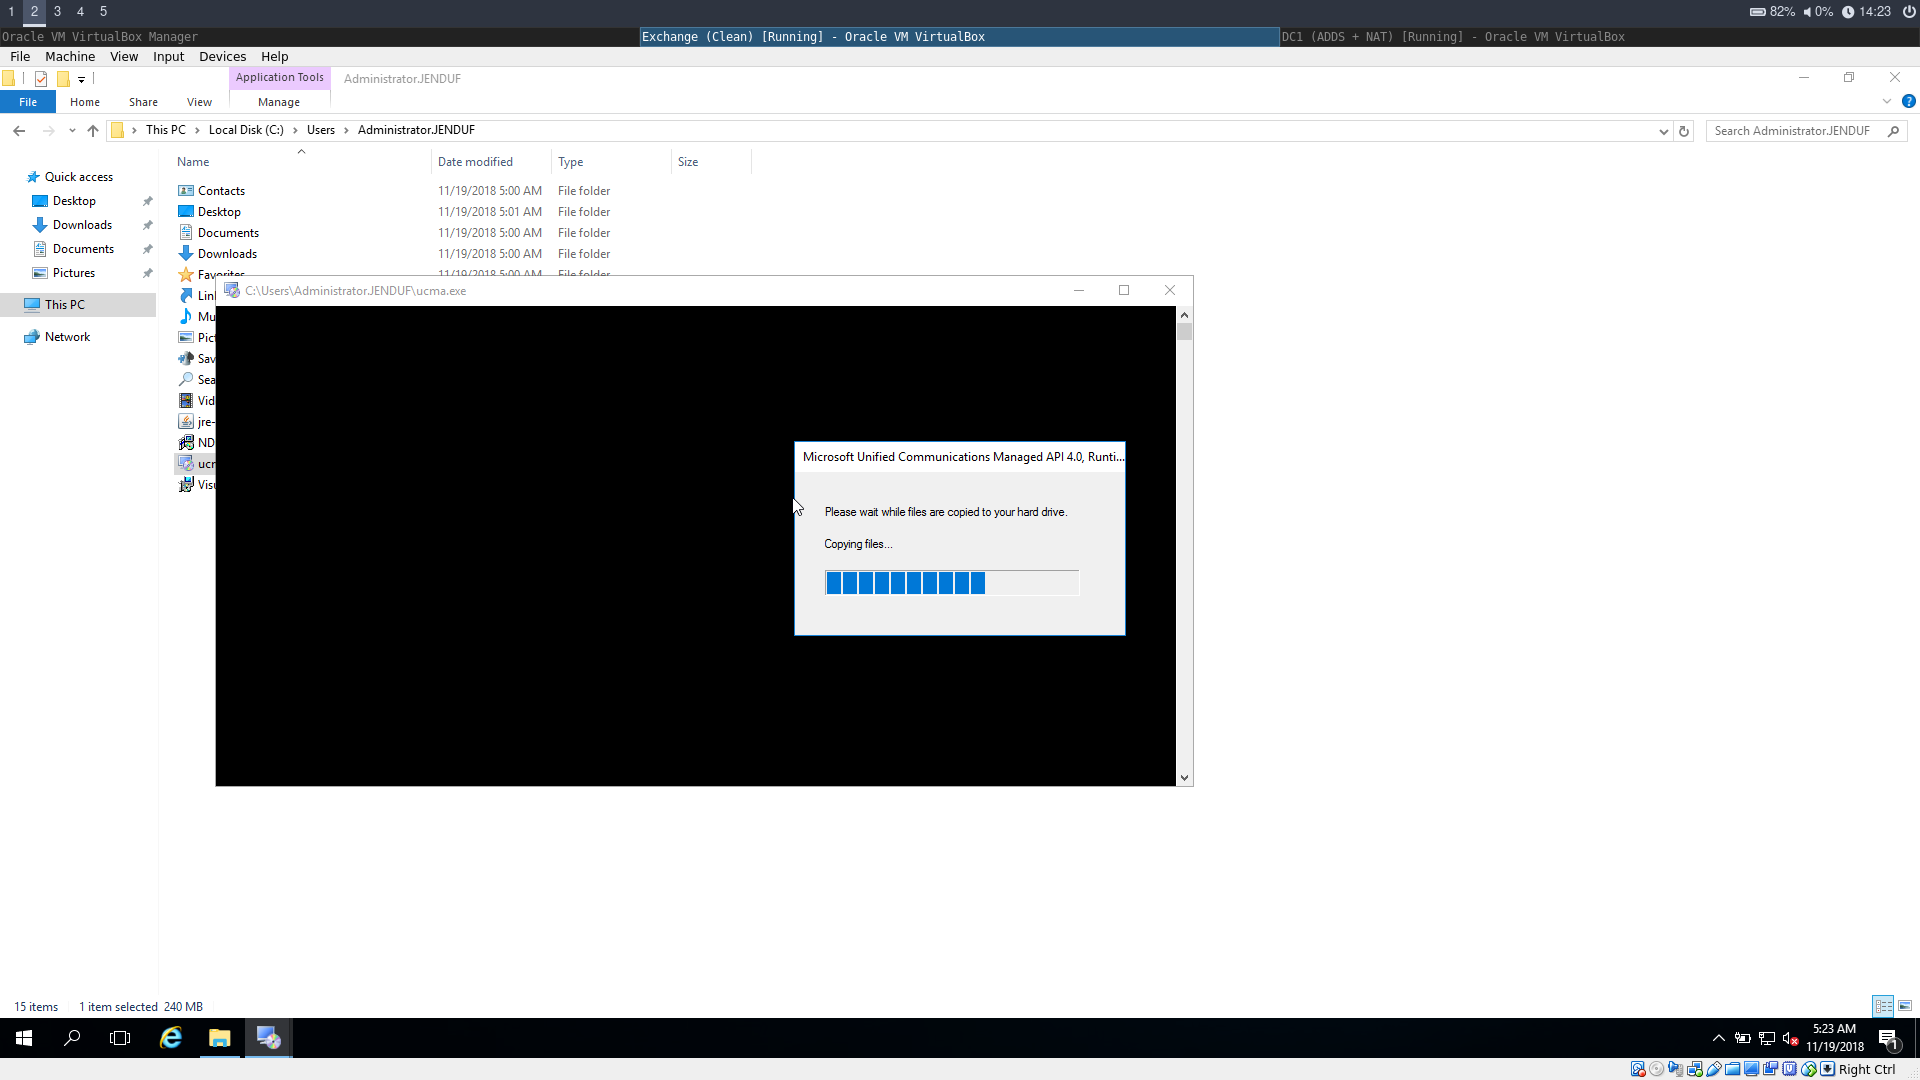
\includegraphics[width=15cm]{Pictures/Exchange/Pre/1542633791.png}
	
	Installeer de "Microsoft Unified Communications Managed API".
\end{center}
	\begin{center}
	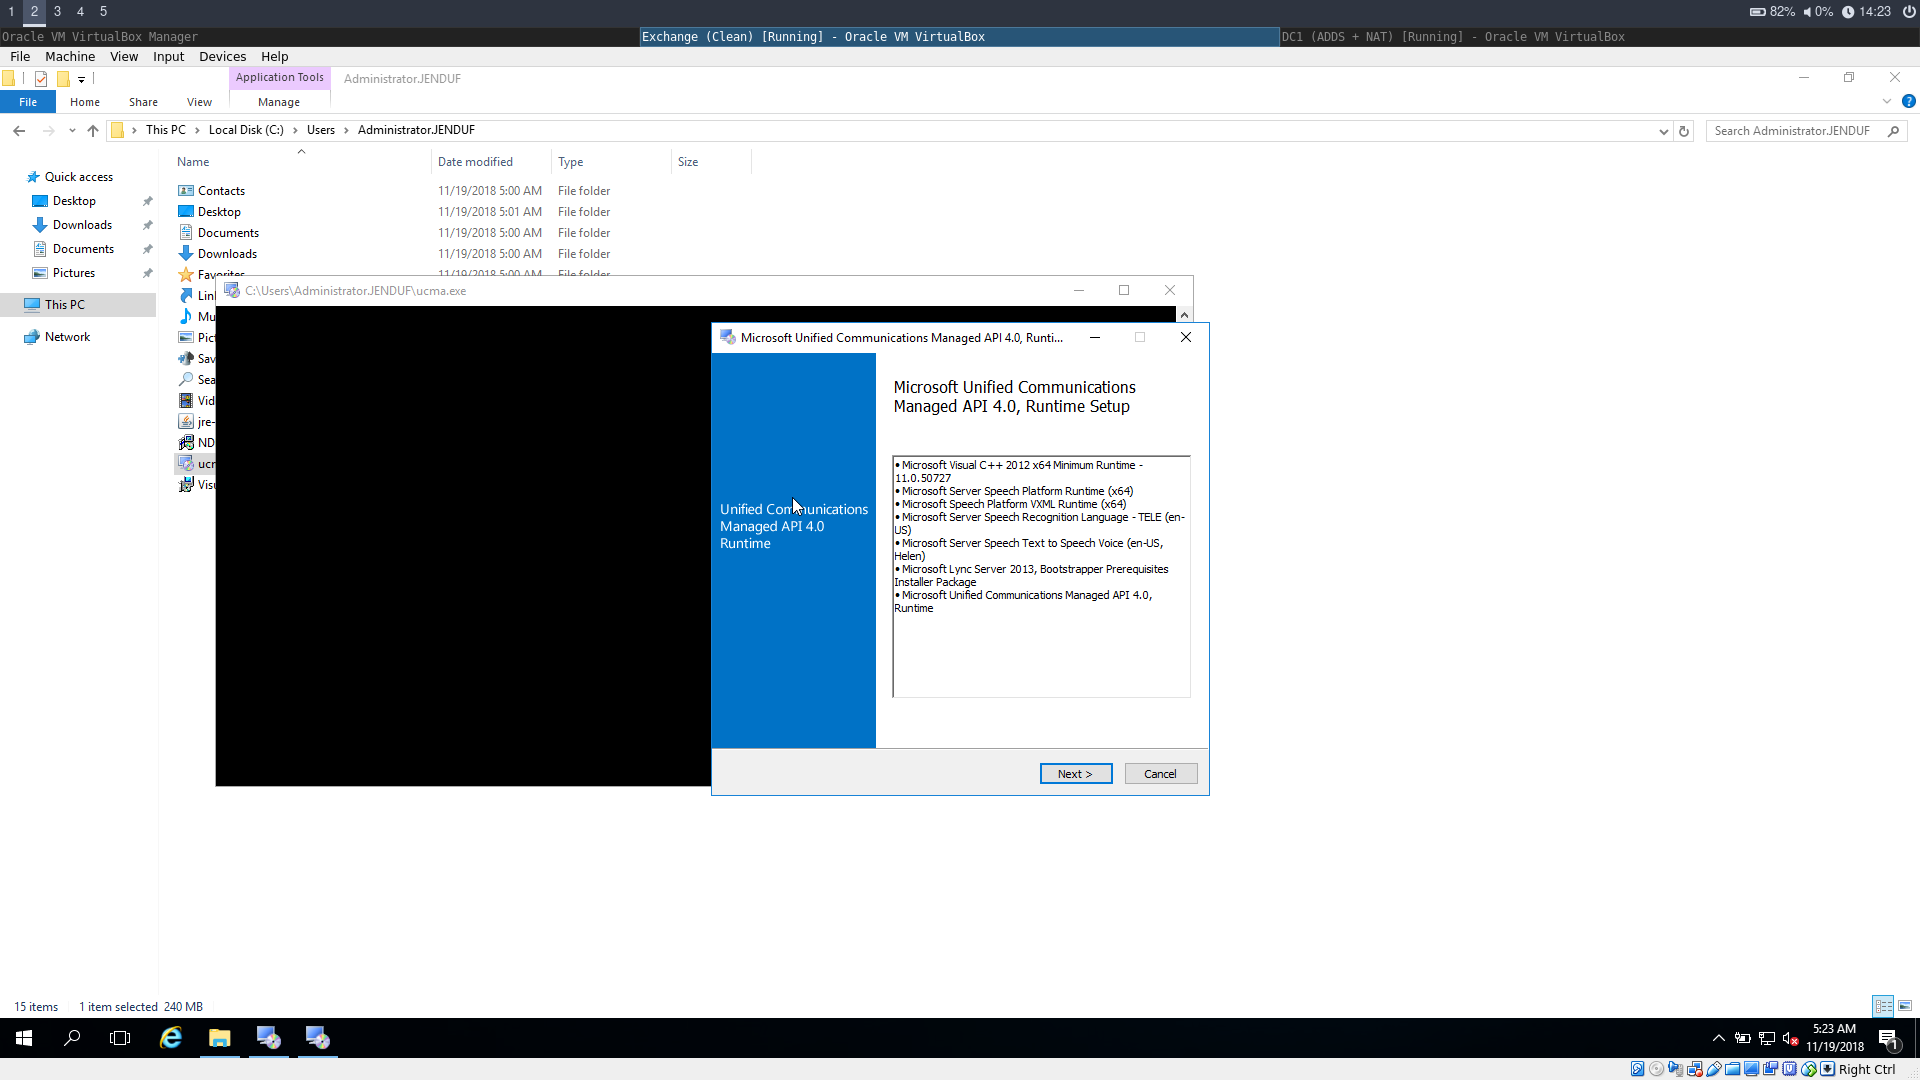
\includegraphics[width=15cm]{Pictures/Exchange/Pre/1542633810.png}
\end{center}
	\begin{center}
	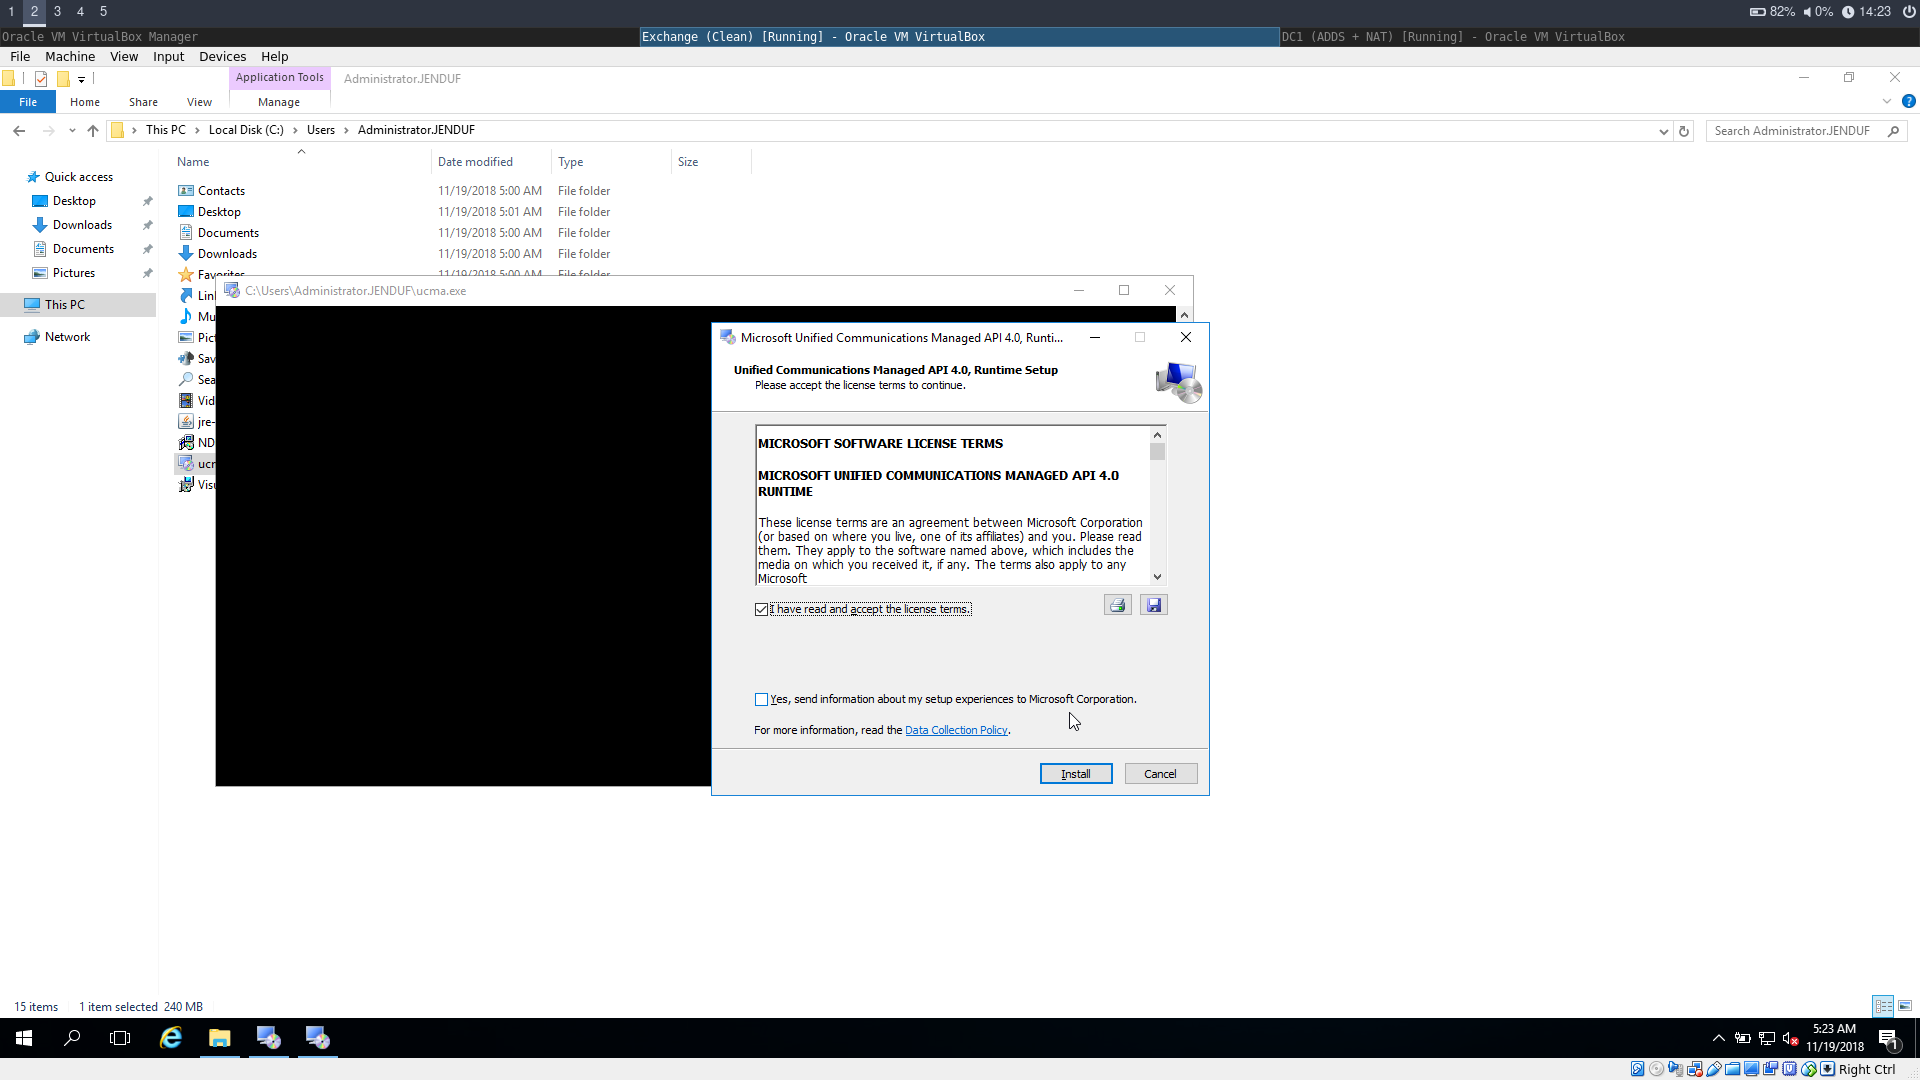
\includegraphics[width=15cm]{Pictures/Exchange/Pre/1542633813.png}
	
	Ga akkoord met de licentievoorwaarden en installeer.
\end{center}
	\begin{center}
	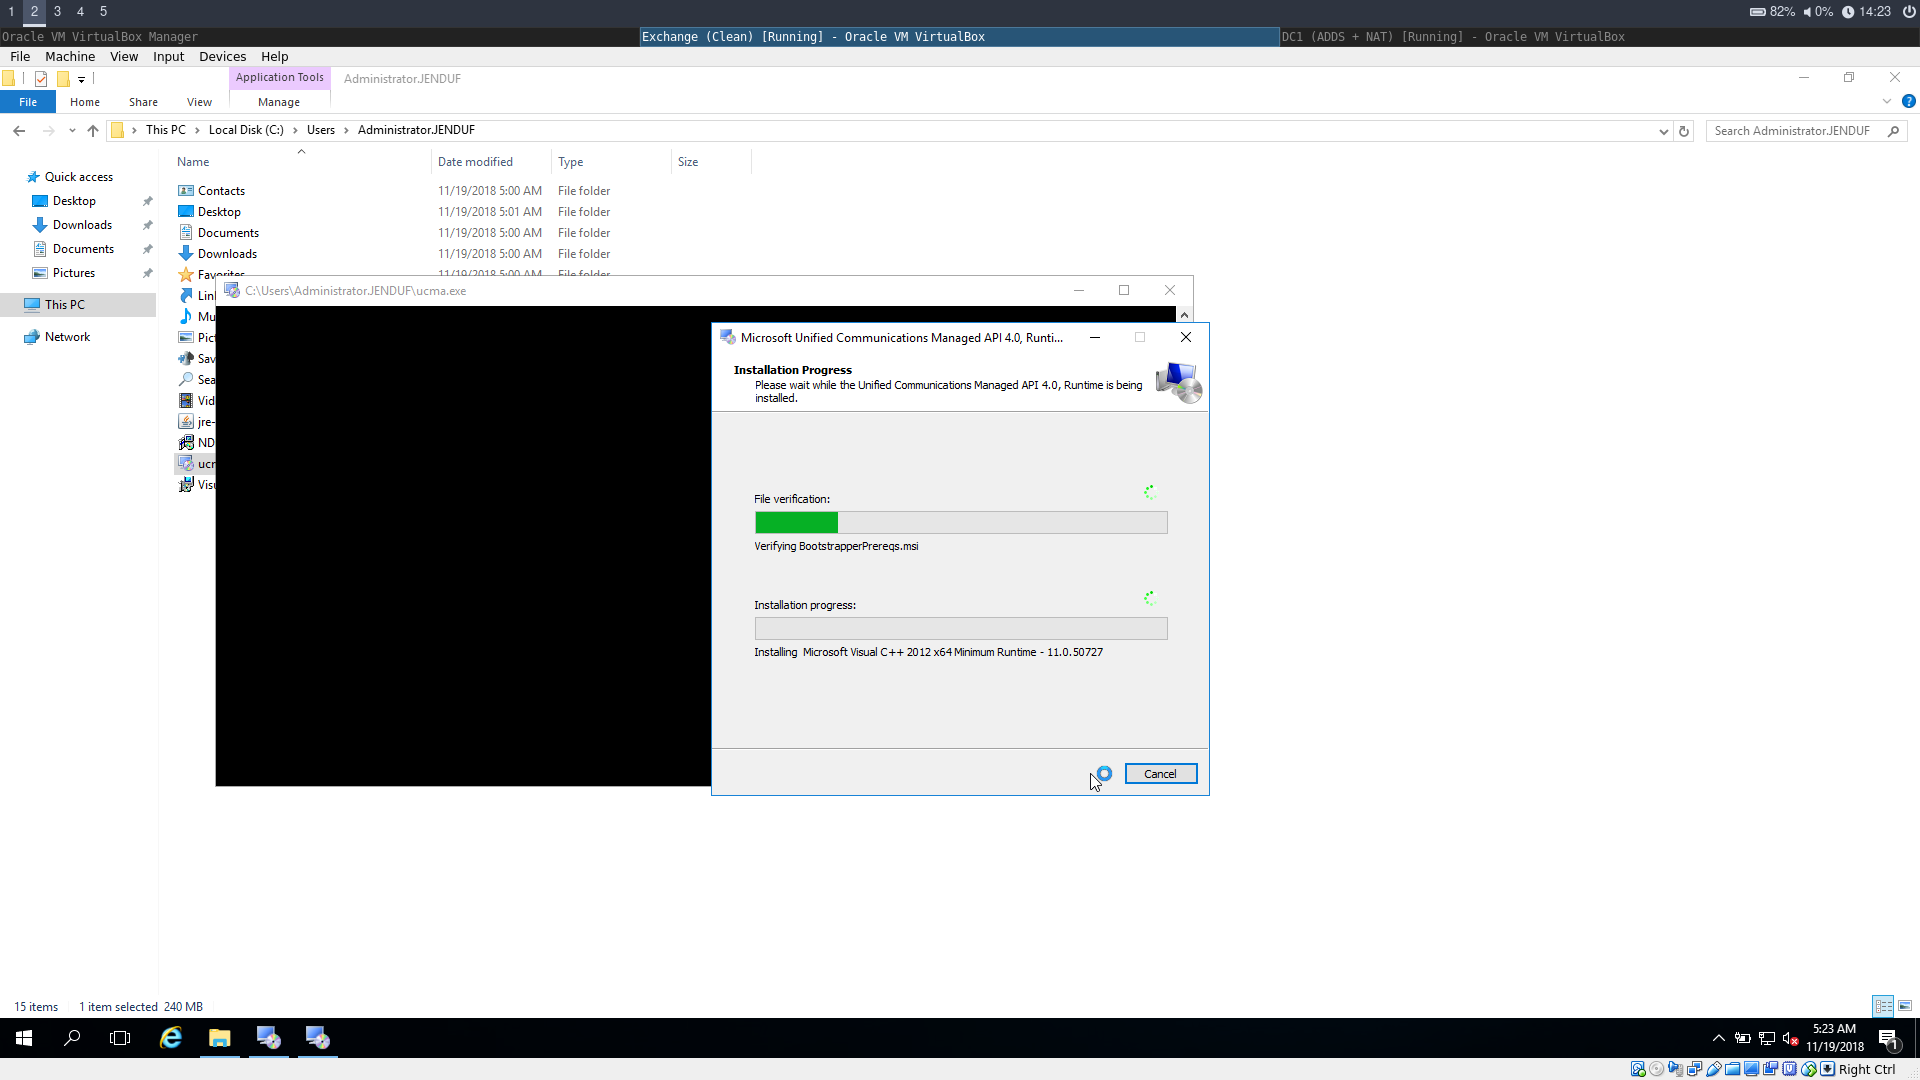
\includegraphics[width=15cm]{Pictures/Exchange/Pre/1542633816.png}
\end{center}
	\begin{center}
	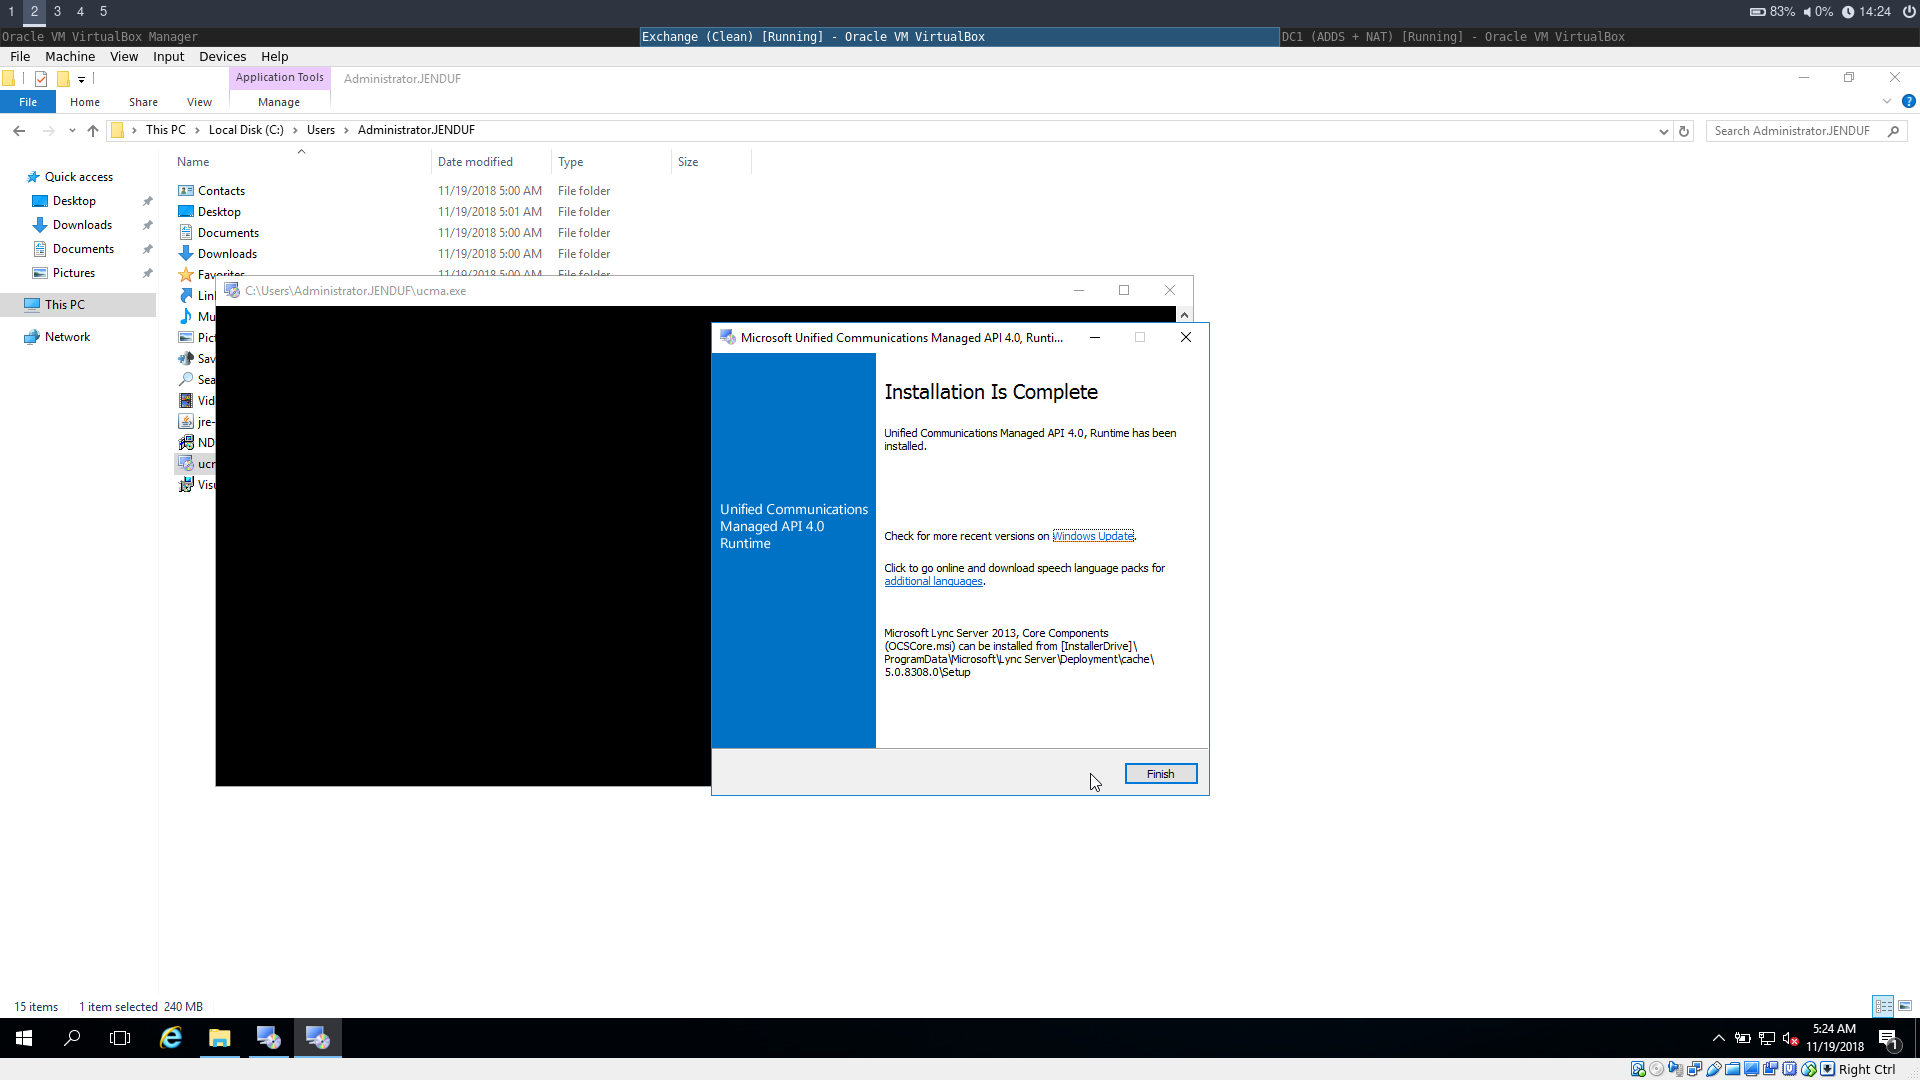
\includegraphics[width=15cm]{Pictures/Exchange/Pre/1542633844.png}
\end{center}
	\begin{center}
	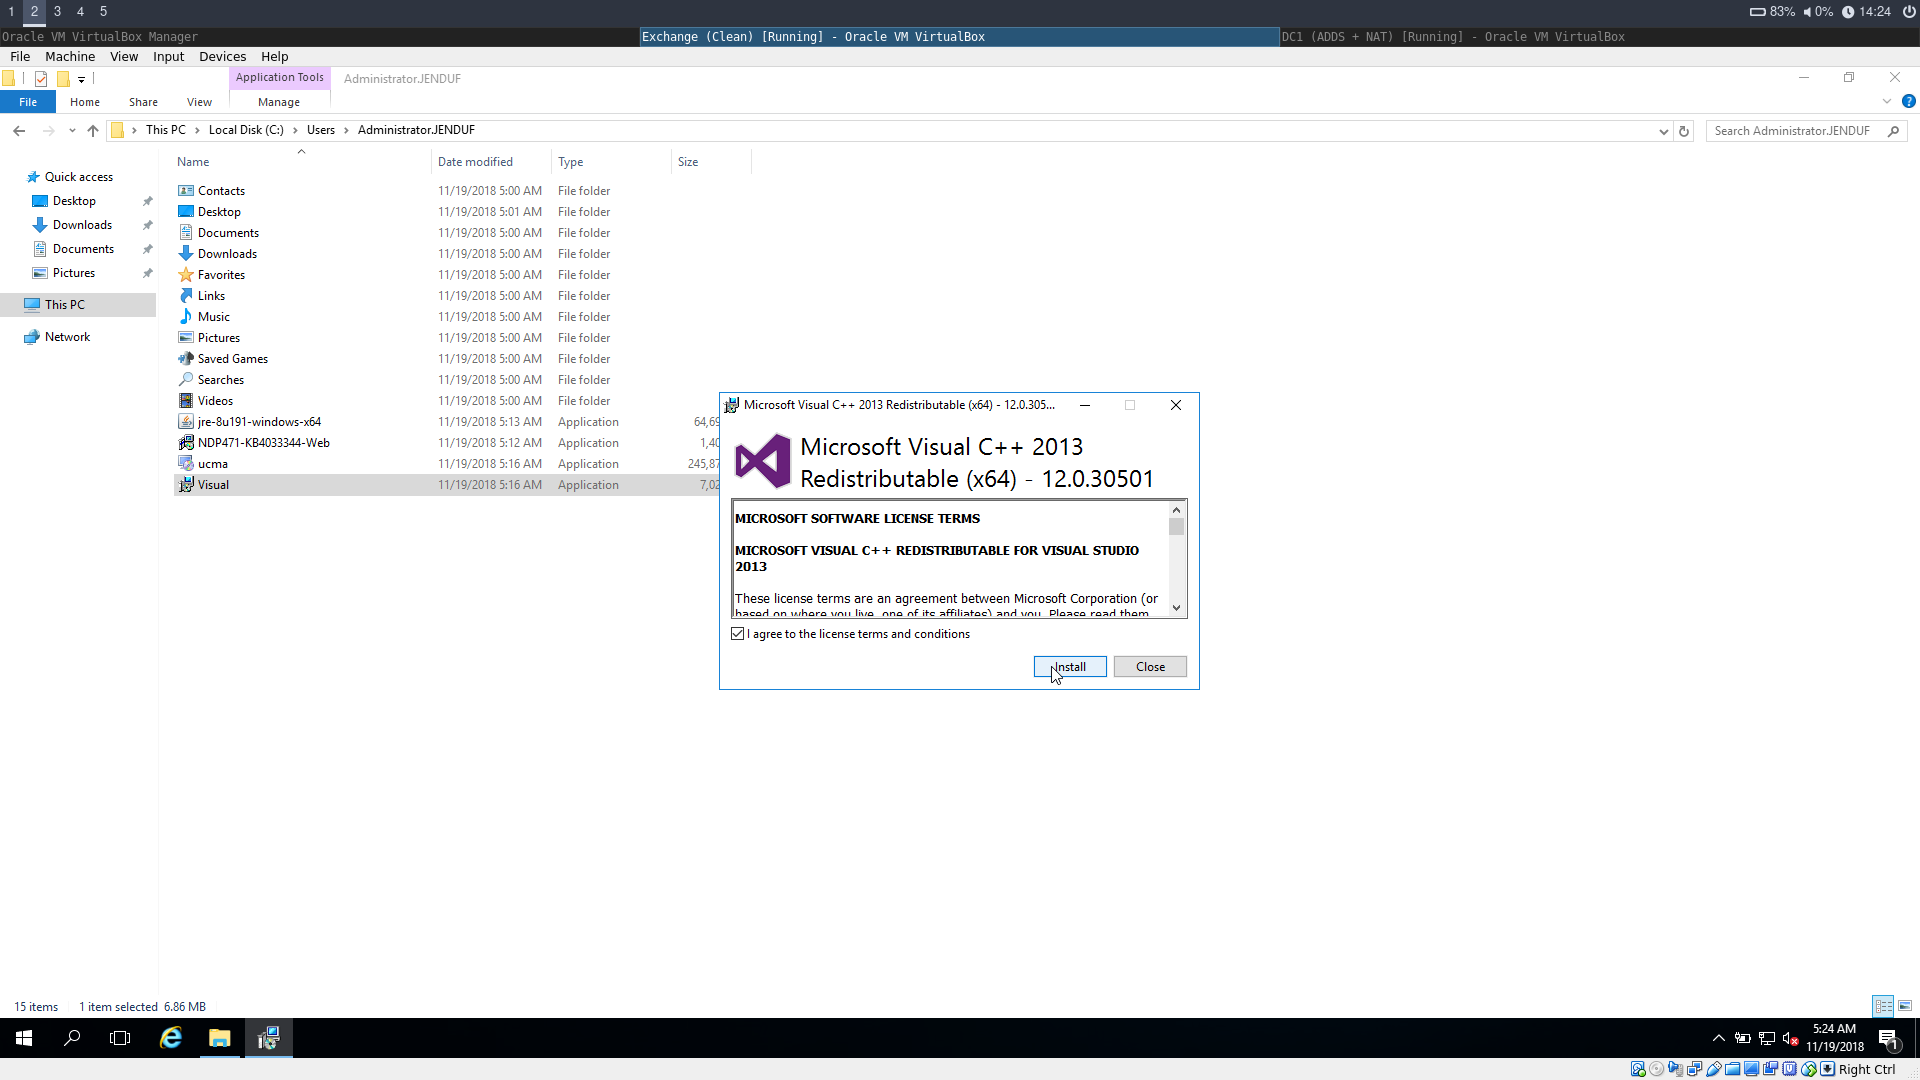
\includegraphics[width=15cm]{Pictures/Exchange/Pre/1542633852.png}
	
	Installeer "Microsoft Visual C++ 2013".
	
\subsection{Installatie Exchange Server}	
\end{center}
\end{document}